\chapter{MATERIAIS E MÉTODOS}
\label{sec:cap4}

%\resumodocapitulo{resumo del capitulo}
\vspace{1cm}

Este capítulo apresenta o desenvolvimento de um sistema de eletroestimulação para exercícios de fortalecimento que incorpora elementos de avaliação automática da atividade neuromuscular. É importante esclarecer que o desenvolvimento e validação dos diferentes módulos que compõem o referido sistema passaram por diversas versões até alcançar a versão aqui descrita. Dessa forma, no Apêndice \ref{ap:ap1} se apresenta detalhes adicionais da evolução do sistema, iniciando com o primeiro eletroestimulador que contava um canal de estimulação e funcionamento limitado, até a versão final que conta com vários canais de estimulação e funcionamento dentro dos parâmetros apresentados na Tabela \ref{tab:c4_rpe1}.


\section{REQUISITOS DO SISTEMA} \label{cap:4_s1}
Como premissa inicial, deve-se levar em consideração que o dispositivo proposto será usado basicamente em quatro ambientes: laboratórios de pesquisa, unidade de tratamento intensivo para pacientes com \acrshort{PNMDC}, clínicas de fisioterapia e por indivíduos com lesão medular. Nesse contexto, o eletroestimulador se encaixa na definição de equipamento eletromédico, e, portanto, é obrigatório no momento do seu projeto a observação da norma geral \acrshort{ABNT} \acrshort{NBR} \acrshort{IEC} 60601-1, que regulamenta acerca de requisitos técnicos mínimos que garantam a segurança operacional destes equipamentos. Além disso, também deve ser observada a norma específica, \acrshort{ABNT} \acrshort{NBR} \acrshort{IEC} 60601-2-10, que adicionalmente à norma geral, apresenta os requisitos particulares para segurança básica e desempenho essencial de estimuladores de nervos e músculos.

Nesse contexto, a Figura \ref{fig:c4_f1_dgd} ilustra um diagrama contendo os componentes principais do sistema proposto. Cada módulo pode ser implementado de diversas formas. Por exemplo a interface de usuário pode ser implementada de forma analógica, digital ou ambas. Aqui se apresenta o requisito final estabelecido para cada módulo. 

A interface de entrada e saída deve ser projetada com a finalidade de controlar o sistema e ao mesmo tempo mostrar informação relevante do processo de do teste de exibilidade e/ou terapia. A interface de controle tem que ser amigável, segura e fácil de se operar por usuários finais que não necessariamente são engenheiros. Neste sistema a interface é projetada para se executar em \acrshort{PC}. A interface, então, deve permitir configurar os parâmetros e rotinas de eletroestimulação, executar início e parada normal ou de emergência da estimulação e, ainda, mostrar informações relacionadas ao funcionamento do eletroestimulador.

O projeto do eletroestimulador começa com o sistema de controle de corrente para a geração do estímulo elétrico. Este, por sua vez, está sujeito à configuração dos parâmetros de estimulação por meio da interface de controle. Assim, o sistema de eletroestimulação proposto, deve contar com um amplo controle e flexibilidade destes parâmetros, assim como robustez em cada módulo que o compõe.

\newpage

%Figura 4.1 – Diagrama geral do dispositivo de eletroestimulação proposto, incluindo (a) alimentação do sistema, (b) interface do usuário, (c) módulo de controle e módulo gerador de sinal, (d) módulo estimulador e (e) módulo de detecção de movimento.
\begin{figure*}
    \centering %
    \small %
    \def\svgwidth{0.9\columnwidth}% Código LATEX define o tamanho da figura 
    \import{figs/Fig_c4/}{c4_f1_dgd.pdf_tex}
    \caption{Diagrama geral do dispositivo de eletroestimulação proposto, incluindo (a) alimentação do sistema, (b) interface do usuário, (c) módulo de controle e módulo gerador de sinal, (d) módulo estimulador e (e) módulo de detecção de movimento.}
    \label{fig:c4_f1_dgd}
\end{figure*}

Os parâmetros de estimulação que o sistema deve atender foram estabelecidos em conjunto com fisioterapeutas das áreas neurológica e \acrshort{UTI} levando em consideração a literatura existente das diferentes aplicações da eletroestimulação em pacientes com lesões e doenças neuromusculares \cite{Silva2016, Carolina2016}. Além disso, foi evidenciada a necessidade de que o sistema de estimulação elétrica possua no mínimo dois canais de saída para poder aplicar estímulos elétricos a  grandes grupos musculares como o quadríceps ou tríceps. Na Tabela \ref{tab:c4_rpe1} são mostrados os valores dos parâmetros de estimulação estabelecidos para o sistema.


% Tabela 4.1 – Requisitos dos parâmetros de estimulação para o novo sistema de eletroestimulação.
% Please add the following required packages to your document preamble:
% \usepackage[table,xcdraw]{xcolor}
% If you use beamer only pass "xcolor=table" option, i.e. \documentclass[xcolor=table]{beamer}
\begin{table}[h]
    \centering
    %\footnotesize
    \caption{Requisitos dos parâmetros de estimulação para o novo sistema de eletroestimulação.}
    \begin{tabular}{|c|c|c|}
    \hline
    \rowcolor[HTML]{D6D6D6} 
    \textbf{Parâmetro físico} & \textbf{Valor ou faixa} & \textbf{Tipo ou unidade} \\ \hline
    Forma de onda (sinal)     & Monofásico / Bifásico   & Quadrada, exponencial.   \\ \hline
    Largura de Pulso          & 100 - 1.106             & $\mathrm{\mu}$s                       \\ \hline
    Frequência                & 0,33 - 150              & Hz                       \\ \hline
    Corrente                  & 1 - 100                 & mA                       \\ \hline
    Carga                     & 100 – 1,5·103           & $\mathrm{\Omega}$                      \\ \hline
    Tempo de terapia          & 0-24                    & h                        \\ \hline
    \end{tabular}
    \label{tab:c4_rpe1}
\end{table}


Da Tabela \ref{tab:c4_rpe1} pode-se observar que o estimulador deve gerar ao menos dois tipos de forma de onda: quadrado e exponencial (em fisioterapia é chamada de exponencial à onda com formato de dente de cerra). Dessa forma, o módulo gerador de sinal (\acrshort{MGS}) deve ser construído visando atender as formas de onda do sinal de estimulação e o controle da mesma, ou seja, o controle deve ser realizado sobre os parâmetros do sinal (que são identificados igualmente como os parâmetros de estimulação) relacionados a geometria da onda, frequência, largura de pulso e amplitude.

Outro componente importante dentro do sistema proposto é o teste de excitabilidade associado a \acrshort{MMG}. Ele, por sua natureza, deve conter um subsistema de detecção de movimento, responsável pela detecção da perturbação mecânica causada por uma contração muscular. Desta forma, os módulos que compõem o \acrshort{MMG} devem ser desenvolvidos visando medir e monitorar as contrações musculares evocadas pelo eletroestimulador no momento da realização do teste de excitabilidade. 

A seguir, são descritas as soluções de hardware e software escolhidas para cada módulo.

\section{HARDWARE}
O hardware do estimulador pode ser identificado como o conjunto dos módulos controle, gerador de sinal, estimulador, detecção de movimento e finalmente, as fontes de alimentação que energizam o sistema completo. Nesse contexto, a prototipagem e desenvolvimento do hardware passou por diversas versões (6 no total, conforme descrito no Apêndice \ref{ap:ap1}) de teste e validação, até chegar na versão aqui apresentada, chamada de versão final. 

Acerca de características gerais, a versão final foi projetada com dois canais de eletroestimulação, onde o canal 1 é usado também de forma integrada ao módulo de detecção de movimento para aplicar o teste de excitabilidade e ajudar na detecção da fadiga. Além disso, um outro aspecto fundamental norteou o desenvolvimento de todos os módulos. Levando em consideração que a realização da eletroterapia continuada pode ter longos períodos de aplicação (até 24 horas), foram escolhidos diferentes componentes eletrônicos com caraterísticas de alto desempenho para implementar o hardware do estimulador. Também foi levado em consideração o isolamento elétrico do circuito do estimulador com a finalidade de evitar correntes de fuga. 

Finalmente, a partir do diagrama apresentado na Figura \ref{fig:c4_f1_dgd}, são descritos de forma detalhada, cada módulo do eletroestimulador proposto.

\subsection{MÓDULO DE CONTROLE}
O módulo de controle ilustrado na Figura \ref{fig:c4_f2_mdc} mostra o esquemático e seus diferentes componentes usados na versão final. Para realizar a função da \acrshort{UC}, foram testados vários sistema embarcado ou plataformas de desenvolvimento tais como o Arduino Mega2560 (microcontrolador ATMega2560, Arduino, Itália) e Teensy 3.2 (microcontrolador MK20DX256VLH7, Freescale, EUA) pela facilidade que apresentam nas provas de conceito e no rápido desenvolvimento do firmware. Elas usam a linguagem \textit{wiring} que é baseada em C/C++ para uma rápida programação de microcontroladores. Também, estas plataformas possuem uma ampla compatibilidade com sensores, módulos de comunicação e diversas interfaces/portas de comunicação, o que possibilitou testar uma ampla gama de soluções relacionadas ao controle e gerenciamento dos recursos do estimulador.

Na versão final do estimulador se escolheu usar dois Teensy 3.2 para conformar a \acrshort{UC}. A principal caraterística desta plataforma é que possui um processador Cortex-M4 de 48MHz (MK20DX256VLH7, Freescale, EUA), várias portas \acrshort{UART}, \acrshort{SPI} e \acrshort{I2C}, entre outras características. Além disso, esta plataforma usa o mesmo \acrshort{IDE} (do inglês \textit{Integrated Development Environment}) que o Arduino.

Nesta etapa de projeto do estimulador não se preocupou com os possíveis atrasos na execução do firmware inerente dessa arquitetura. De fato, ao usar a linguagem \textit{wiring}, o código binário possui pequenas redundâncias que podem consumir um certo número de ciclos de processador a mais. Testes posteriores devem validar o desempenho do sistema.

Para à interação entre o estimulador (\acrshort{UC}) e o usuário, foi escolhido implementar uma interface de controle com comunicação bidirecional para ser executada em \acrshort{PC} via \acrshort{USB}.

Como é evidenciado na Figura \ref{fig:c4_f2_mdc}, a \acrshort{UC} possui dois Teensy 3.2: $\mathrm{\mu}$C1\_STIM e $\mathrm{\mu}$C2\_ACEL. O $\mathrm{\mu}$C1\_STIM possui então as seguintes tarefas: gerenciar a comunicação de entrada e saída via \acrshort{USB} e Bluetooth para futuras aplicações; comunicar-se com o \acrshort{DAC} do módulo gerador de sinal via \acrshort{SPI} para gerar o sinal de referência do estímulo (\acrshort{SPI}); realizar o chaveamento entre a ativação da saída do canal e a pré-carga no módulo de estimulação (RELAY\_CHX) conforme a descrição na Seção 4.2.6; comunicar-se com o $\mathrm{\mu}$C2\_ACEL; e, por fim, verificar o estado do botão de emergência (BTN EMERGÊNCIA). O gerenciamento destas funções é governado pelo firmware, o qual é explicado no item 4.3.1. O $\mathrm{\mu}$C2\_ACEL é responsável por gerenciar o sensor inercial do módulo de detecção de movimento.

%Figura 4.2 – Módulo de controle, diagrama esquemático do módulo de controle.
\begin{figure*}[h]
    \centering %
    \scriptsize %
    \def\svgwidth{0.61\columnwidth}% Código LATEX define o tamanho da figura 
    \import{figs/Fig_c4/}{c4_f2_mdc.pdf_tex}
    \caption{Módulo de controle, diagrama esquemático do módulo de controle.}
    \label{fig:c4_f2_mdc}
\end{figure*}

Finalmente, para energizar os componentes que fazem parte do módulo de controle é necessária uma fonte de alimentação de 5$V_{DC}$ com no mínimo 500mA. É de esclarecer que existem dois tipos de terras isoladas sendo elas GND\_D e GND\_HV, terra da parte digital e terra da parte de alta tensão respectivamente. Assim, tanto o $\mathrm{\mu}$C1\_STIM quanto o $\mathrm{\mu}$C2\_ACEL compartem o mesmo aterramento GND\_D. A escolha da fonte e outras discussões relativas são descritos no item 4.2.5. 

\subsection*{Circuito de isolamento}
A norma \acrshort{ABNT} \acrshort{NBR} \acrshort{IEC} 60601-1 prevê provas de segurança elétrica para determinar se o equipamento eletromédico possui correntes de fuga. A corrente de fuga é o termo usado para indicar um fluxo de corrente anormal ou indesejada em um circuito elétrico devido a uma fuga (geralmente um curto-circuito ou a um caminho anormal de baixa impedância). 

Agora, dentro do estimulador existem tensões baixas e altas e correntes que podem chegar até os 150mA. O circuito de isolamento permite isolar o módulo de controle que funciona com tenções de no máximo 5$V_{DC}$ do resto do circuito que funciona com 15$V_{DC}$ e 160$V_{DC}$ se considerando como alta tensão. Isto é feito com intuito de evitar possíveis correntes de fuga que possam circular entre acessórios\footnote{Acessório em sistemas eletromédicos são identificados como “partes aplicadas” segundo a norma geral \acrshort{ABNT} \acrshort{NBR} \acrshort{IEC} 60601-1 no item de Segurança elétrica.}  conectados ao estimulador e o paciente, entre o gabinete do estimulador ou do computador (por causa \acrshort{USB} compartindo a terra) e o paciente. 

O ponto em que é feito o isolamento acontece na comunicação \acrshort{SPI} entre $\mathrm{\mu}$C1\_STIM do módulo de controle e o \acrshort{DAC} do módulo gerador de sinal. Para esta tarefa foi escolhido o \acrshort{CI} ISO7240C (Texas Instrument, USA) que proporciona um isolamento digital unidirecional de quatro vias de até 4kV. Usado em conjunto com fontes de alimentação isoladas, este dispositivo ajuda a bloquear altas tensões, isolar aterramentos e impedir que ruído eletrônico entrem no aterramento e interfiram ou danifiquem os circuitos sensíveis.

A Figura \ref{fig:c4_f3_iso} mostra o esquemático com as conexões do circuito de isolamento. Nele são usadas duas fontes, cada uma com 5$V_{DC}$ e terras separadas GND\_D e GND\_HV. 

\vspace{0.3cm}
% Figura 4.3 – Diagrama esquemático do circuito de isolamento ISO7140C e suas conexões.
\begin{figure*}[h]
    \centering %
    \small %
    \def\svgwidth{0.7\columnwidth}% Código LATEX define o tamanho da figura 
    \import{figs/Fig_c4/}{c4_f3_iso.pdf_tex}
    \caption{Diagrama esquemático do circuito de isolamento ISO7140C e suas conexões.}
    \label{fig:c4_f3_iso}
\end{figure*}

\subsection{MÓDULO GERADOR DE SINAL} \label{cap:sec4.2.2}
Antes de escolher a solução final do \acrshort{MGS} da versão final, foram testadas várias outras topologias do circuito responsável pela geração do sinal, como os circuitos integrados (\acrshort{CI}) geradores de sinal (e.g. ICL8038 e XR2206), microcontroladores e plataformas de desenvolvimento programados para modular um sinal por largura de pulso (\textit{Pulse Width Modulation}, \acrshort{PWM}) e, finalmente, conversores digitais-analógicos ou \acrshort{DAC}s.

As soluções com \acrshort{CI}s e \acrshort{PWM} foram descartados pela complexidade na montagem e controle dos mesmos na hora de gerar os sinais. Nas topologias com os \acrshort{CI}s, em alguns casos, é necessário trocar componentes físicos (notadamente capacitores) para se alterar a frequência de operação. Já no uso de \acrshort{PWM} era necessário gerar vários sinais desse tipo para formar um sinal bifásico (como ilustrado na Figura \ref{fig:onb_f6}), sendo que ao mesmo tempo em alguns casos a solução iria consumir mais tempo de processamento do microcontrolador apenas para esta tarefa específica. Por último, foi testada a solução com \acrshort{DAC}, escolhida pela facilidade de controle e comunicação \acrshort{SPI} de 3 vias para gerar os sinais do estimulador. Note-se que o gerador de sinais baseado no \acrshort{DAC} é muito mais versátil que com os \acrshort{CI}s e \acrshort{PWM}, pois ele permite criar qualquer forma de onda e oferece um controle simplificado dos parâmetros relacionados com ela. A partir do uso de tal solução, pode-se inclusive gerar sinais arbitrários de eletroestimulação.

Nessa ordem de ideias, foram testados seis \acrshort{DAC}s, os quais são caraterizados na Tabela \ref{tab:c4_dac2}. Nela são mostradas as referências e caraterísticas de cada um deles.

% Tabela 4.2 –Caraterísticas dos DACs testados para o MGS.
% Please add the following required packages to your document preamble:
% \usepackage[table,xcdraw]{xcolor}
% If you use beamer only pass "xcolor=table" option, i.e. \documentclass[xcolor=table]{beamer}
\begin{table}[h]
    \centering
    \small
    \caption{Caraterísticas dos DACs testados para o MGS.}
    \begin{tabular}{|c|c|c|c|c|c|}
    \hline
    \rowcolor[HTML]{D6D6D6} 
    \textbf{\begin{tabular}[c]{@{}c@{}}Referência do \\ DAC\end{tabular}} & \textbf{\begin{tabular}[c]{@{}c@{}}Canais \\ D/A\end{tabular}} & \textbf{\begin{tabular}[c]{@{}c@{}}Bits de \\ conversão\end{tabular}} & \textbf{\begin{tabular}[c]{@{}c@{}}Tensão de saída \\ do canal (VDC)\end{tabular}} & \textbf{\begin{tabular}[c]{@{}c@{}}Porta de \\ comunicação\end{tabular}} & \textbf{Fabricante}    \\ \hline
    MCP4921                                                               & 1                                                              & 12                                                                    & 5                                                                                  & SPI                                                                      & Microchip              \\ \hline
    MCP4922                                                               & 2                                                              & 12                                                                    & 5                                                                                  & SPI                                                                      & Microchip              \\ \hline
    DAC121S101                                                            & 1                                                              & 12                                                                    & 5                                                                                  & I2C                                                                      & National Semiconductor \\ \hline
    DAC124S085                                                            & 4                                                              & 12                                                                    & 5                                                                                  & SPI                                                                      & Texas Instruments      \\ \hline
    DAC128S085                                                            & 8                                                              & 12                                                                    & 5                                                                                  & SPI                                                                      & Texas Instruments      \\ \hline
    DAC8718SPAG                                                           & 8                                                              & 16                                                                    & $\mathrm{\pm}$15                                                                               & SPI                                                                      & Texas Instruments      \\ \hline
    \end{tabular}
    \label{tab:c4_dac2}
\end{table}

Inicialmente foi trabalhado o MCP4921 da Microchip. Ele possui um canal de conversão digital-analógico (\acrshort{DA}) de 8 bits e é controlado via \acrshort{SPI}. O MCP4922 possui dois canais \acrshort{DA} e as mesmas caraterísticas do anterior com relação à conversão e comunicação. Esses dois \acrshort{DAC}s permitiram testar e implementar um firmware inicial para a criação de sinais quadrados e gerenciamento dos mesmos. Esses \acrshort{DAC}s, porém, não foram usados devido à quantidade de canais que ofereciam em único chip, pois nos requisitos do sistema foi evidenciada a necessidade de 2 canais. Mesmo havendo a possibilidade de se usar vários deles, isto faria com que o circuito em geral tivesse um maior tamanho. Dessa forma, foram buscadas outras soluções de encapsulamento, seja \acrshort{THM} (do inglês Through Hole Mounting) ou preferencialmente \acrshort{SMD} (do inglês Surface Mount Device).

Foi explorado então outro DAC, o DAC121S085 \acrshort{SMD}, que possui uma taxa de conversão mais rápida quando comparado com o MCP4921/2, porém só apresenta um canal \acrshort{DA}. Por esta razão, foram usados os \acrshort{DAC}s DAC124S085 e DAC128S085 com 4 e 8 canais de conversão \acrshort{DA}, respectivamente. Com eles foi possível testar o gerenciamento de recursos na geração do sinal em cada canal de forma independente, permitindo evidenciar a dificuldade disto com relação ao consumo de recursos na \acrshort{UC}. 

Como pode ser observado na Tabela \ref{tab:c4_dac2}, o único \acrshort{DAC} que possui canais DA com saída bipolar é o DAC8718SPAG \acrshort{SMD}. Este \acrshort{DAC} é de uso militar e, devido a essa e outras caraterísticas, seu preço é dez vezes mais caro quando comparado com os outros \acrshort{DAC}s similares. Além disso, o controle para o uso de seus recursos resultou ser complicado, pois além do componente de software, é preciso usar componentes eletrônicos adicionais para seu correto funcionamento. Tais características o eliminaram da escolha final do \acrshort{DAC} que faz parte do \acrshort{MGS}. Portanto, pela disponibilidade e quantidade de canais de conversão, escolheu-se o DAC124S085, que com seus 4 canais de conversão \acrshort{DA} a uma resolução de 12 bits, comunicação via \acrshort{SPI} de três cabos e uma taxa de conversão de 1 \acrshort{MSPS} (do inglês Million Samples Per Second) cumpre os requisitos do sistema. Com ele foram implementados vários circuitos em \acrshort{PCI}, os quais podem ser evidenciados no Apêndice I.  É de esclarecer que na versão final do eletroestimulador só foram usados dois canais do \acrshort{DAC}, mas é possível implementar os outros seguindo a mesma topologia do circuito descrita para o canal um e dois.

\subsection*{Topologia e saída de tensão do circuito Gerador de Sinal}
O circuito esquemático descrito na Figura \ref{fig:c4_f4_msg}, apresenta a topologia do gerador de sinal baseado no DAC124S085 da versão final do sistema de estimulação. Como pode-se observar, o DAC124S085 se comunica com o Teensy 3.1 por meio da porta \acrshort{SPI}. Para alimentar o \acrshort{DAC} é usada uma fonte regulada de 4,096$V_{DC}$ de alta precisão baseada no regulador LM4132 (Texas Instruments, EUA). Ele fornece uma alta estabilidade na saída dos canais do conversor \acrshort{DA}. Desta forma, a mesma fonte que energiza o \acrshort{DAC} é usada como tensão de referencia ($V_{ref}$) dos canais do mesmo.

%Figura 4.4 – Diagrama esquemático do MGS, no qual é mostrado em destaque circuito para gerar sinal bifásico a partir de referência monofásica.

\begin{figure*}[h]
    \centering %
    \tiny %
    \def\svgwidth{1\columnwidth}% Código LATEX define o tamanho da figura 
    \import{figs/Fig_c4/}{c4_f4_msg.pdf_tex}
    \caption{Diagrama esquemático do \acrshort{MGS}, no qual é mostrado em destaque circuito para gerar sinal bifásico a partir de referência monofásica.}
    \label{fig:c4_f4_msg}
\end{figure*}

O \acrshort{DAC} tem uma resolução de 12 bits para conversão. Manipulando o valor da conversão (usando o sistema de numeração decimal) é possível criar qualquer formato de onda monofásico, como exemplificado na Figura \ref{fig:c4_f5_fon}, onde a geometria da onda obedece diferentes valores decimais que representam uma amplitude de tensão que depende de $V_{ref}$. Por exemplo, com $V_{ref}$ = 4,096$V_{DC}$, temos que cada variação de unidade decimal ($\Delta V$) equivale a $\Delta V= \frac{V_{ref}}{12bits}=1mV$.

É importante ressaltar que o DAC124S085 funciona somente com valores de tensão positivos (usando $V_{ref}$) o que configura um funcionamento só para sinais monofásicos. Portanto para gerar um sinal bifásico é preciso usar adicionalmente outro circuito ou arquitetura que, a partir do sinal criado pelo conversor ($V_{OUTA}$ para o canal 1 do \acrshort{DAC}), seja gerado o sinal bifásico. Para isto é usada a topologia do amplificador diferencial (i.e. subtrator) de tensão utilizando amplificador operacional \cite{Jung2005, Carter2001}. 

Na Figura \ref{fig:c4_f4_msg}, a caixa pontilhada de cor laranja apresenta a topologia do circuito diferencial de tensão composto pelo amplificador operacional U1A e os resistores $R_1$ e $R_2$. Nele, há dois sinais de entrada: a tensão de referência ($V_{ref}$) pelo resistor $R_1$ (entrada inversora) e uma das saídas \acrshort{DAC} ($V_{OUTA}$ na entrada não inversora). É de esclarecer que na Figura \ref{fig:c4_f4_msg} está evidenciado como exemplo só o conjunto de componentes eletrônicos de um canal ($V_{OUTA}$), pois os demais canais seguem e/ou replicam a mesma topologia. 

A partir do $V_{OUTA}$, o amplificador diferencial cria o sinal bifásico. Tomando como exemplo o canal um, então, temos que o sinal de saída ($S_{OUT}$ na Figura \ref{fig:c4_f4_msg}) é descrita pela seguinte equação,

% Figura 4.5 – Formas de onda monofásicas que podem ser criadas pelo DAC do MGS.
\begin{figure*}[h]
    \centering %
    \small %
    \def\svgwidth{1\columnwidth}% Código LATEX define o tamanho da figura 
    \import{figs/Fig_c4/}{c4_f5_fon.pdf_tex}
    \caption{Formas de onda monofásicas que podem ser criadas pelo \acrshort{DAC} do \acrshort{MGS}.}
    \label{fig:c4_f5_fon}
\end{figure*}

% eQUA~]AO 4.1
\begin{equation}
    S_{OUT} =\left(V_{ref} \cdot \left(\frac{\Delta V}{12bits}\right)\cdot\left(\frac{(R_1 + R_2)}{R_1}\right)\right)- V_{ref}\cdot\frac{R_2}{R_1}
    \label{eq:c4_1}
\end{equation}

onde $S_{OUT}$ é saída do amplificador diferencial equivalente ao sinal bifásico; $\Delta V$ representa a variação decimal ou código de entrada decimal, o qual é gerenciado pelo $\mathrm{\mu}$C1\_STIM da \acrshort{UC} e, finalmente, a tensão de referência, $V_{ref}$.

Além do anterior, no caso do estimulador proposto neste trabalho, a topologia do diferencial requer que o amplificador operacional (U2A na Figura \ref{fig:c4_f4_msg}) seja polarizado com uma fonte simétrica em uma faixa de tensão de $\mathrm{\pm}$15v e que os valores de $R_1$ e $R_2$ sejam exatamente iguais. Isto com a finalidade de criar um sinal bifásico simétrico. Com estas condições, a equação (\ref{eq:c4_1}) é simplificada na equação (\ref{eq:c4_2}), a seguir,

% EQUAÇÃO 4.2
\begin{equation}
    S_{OUT} =\left(
2 \cdot V_{ref} \cdot 
\left(
\frac{\Delta V}{12bits}\right)\right)- V_{ref}
\label{eq:c4_2}
\end{equation}

Como mencionado, manipulando os valores de $\Delta V$ é possível criar qualquer sinal com forma de onda monofásica. Basicamente, o valor referente à terra ou \textit{ground} (\acrshort{GND}) é um $\Delta V$ constante igual a 2047 ou 6bits. A Figura 4.6 (b) mostra um exemplo de sinal quadrado simétrico, onde $\Delta V$ tem valor máximo positivo de 4095, equivalente a $\frac{V_{ref}}{2}$, o máximo negativo com valor igual a 0, equivalente a $\frac{-V_{ref}}{2}$ e \acrshort{GND} com 2047. Desta forma é gerando o sinal bifásico simétrico (b) a partir do sinal monofásico (a). 

Assim, o sinal bifásico simétrico $S_{OUT}$ (Figura 4.6 (b)) possui uma amplitude máxima de $\frac{\mathrm{\pm} V_{ref}}{2}$, ou seja, como $V_{ref}$  é 4,096$V_{DC}$ a amplitude máxima de tensão de cada fase é 2,048$V_{DC}$ . Essas amplitudes vão representar então, a corrente máxima do estímulo, ou seja, 4,096$V_{DC}$  = +100mA e 0$V_{DC}$  = -100mA.

Agora, se realizamos um exercício onde se seleciona $\mathrm{\pm}$1mA, temos que o sinal teria uma amplitude de 20,48m$V_{DC}$. No entanto, esse valor de tensão se encontra dentro da amplitude de ruído inerente das saídas do \acrshort{DAC}. Portanto, a relação sinal-ruído deve ser melhorada. Para isto o $S_{OUT}$  é condicionado, adicionando um circuito eletrônico de amplificação para elevar a tensão. O valor máximo de amplificação depende do módulo estimulador, especificamente do conversor de tensão-corrente que usa um resistor de precisão para a referida tarefa. Nesse contexto, é usada a topologia do amplificador não inversor para elevar a tensão de $S_{OUT}$  até um valor de $\mathrm{\pm}12S_{OUT}$, de acordo com o descrito na Seção 4.2.3. 
%%%%%%%%%%%%%%%%%%%%%%%%%%%%%%%%%%%%%%%%%%%%%%

% Figura 4.6 – Sinal para ilustrar funcionamento do MGS, em especial o sinal monofásico VOUTA (a) e sinal bifásico SOUT (b).
\begin{figure*}
    \centering %
    \small %
    \def\svgwidth{1\columnwidth}% Código LATEX define o tamanho da figura 
    \import{figs/Fig_c4/}{c4_f6_mab.pdf_tex}
    \caption{Sinal para ilustrar funcionamento do \acrshort{MGS}, em especial o sinal monofásico $V_{OUTA}$ (a) e sinal bifásico $S_{OUT}$ (b).}
    \label{fig:c4_f6_mab}
\end{figure*}

A Figura \ref{fig:c4_f7_amd} mostra o esquemático do circuito que amplifica o $S_{OUT}$ do primeiro canal do \acrshort{DAC}, configurando a saída do estímulo do canal 1: $S_{CH1}$. É de aclarar que foi usado o \acrshort{CI} TL084 que possui 4 amplificadores operacionais (U1A, U1B, U1C, U1D), onde U1A e U1B é utilizado na implementação do amplificador diferencial. Também, vale ressaltar que o $S_{CH2}$ possui a mesma topologia. Por outro lado, com relação a $R_1$, o valor escolhido foi de 1k$\mathrm{\Omega}$ e o $VR_1$ 2k$\mathrm{\Omega}$ foi ajustado ao mesmo valor de $R_1$, seguindo as recomendações do fabricante do \acrshort{DAC} para a operação bipolar e, para realizar a amplificação, o valor de $R_2$ = 1k$\mathrm{\Omega}$ e $VR_2$ $\mathrm{\approx}$4,86k$\mathrm{\Omega}$ o que oferece um ganho de 5,86 levando o sinal ao valor requerido de $\mathrm{\pm}12V_{DC}$. Fisicamente foram usados potenciômetros de precisão (\textit{trimpots} de $\mathrm{\pm}$1\% de tolerância) para ajustar o valor fixo de $VR_1$ e $VR_2$ e, para $R_1$ e $R_3$ foram utilizados resistores de precisão de $\mathrm{\pm}$1\% de tolerância.

\vspace{0.3cm}
% Figura 4.7 – Diagrama esquemático do amplificador diferencial para gerar SOUT e o circuito amplificador subsequente para gerar a saída SCH1.
\begin{figure*}[h]
    \centering %
    \small %
    \def\svgwidth{0.9\columnwidth}% Código LATEX define o tamanho da figura 
    \import{figs/Fig_c4/}{c4_f7_amd.pdf_tex}
    \caption{Diagrama esquemático do amplificador diferencial para gerar $S_{OUT}$ e o circuito amplificador subsequente para gerar a saída $S_{CH1}$.}
    \label{fig:c4_f7_amd}
\end{figure*}

% new section %%%%%%%%%%%%%%%%%%%%%%%%%%%%%%
\subsection{MÓDULO ESTIMULADOR}
 
Uma das escolhas realizadas inicialmente neste trabalho foi realizar a eletroestimulação usando sinais de corrente. Desta forma, o módulo do estimulador é responsável por manter uma corrente fixa em uma carga variável, ou seja, neste módulo é especificado um valor de corrente (corrente de referência ou $I_{ref}$) que será entregue ao conjunto tecido-eletrodo (carga) do paciente a ser eletroestimulado. A referida corrente é controlada a partir do sinal $S_{CHx}$ (onde x representa o canal 1 e 2) proveniente do módulo gerador de sinal. Nesse contexto, o módulo estimulador é composto por dois circuitos: um conversor de tensão-corrente e um estágio de potência (\acrshort{EP}), os quais são descritos a seguir.


\subsection*{Topologia do circuito conversor de tensão-corrente}
O conversor de tensão-corrente é um circuito que segue a topologia da arquitetura de \textit{Howland} com retroalimentação negativa. Neste, o sinal de tensão $S_{CHx}$ do módulo gerador de sinal é convertido em um sinal de corrente formando a corrente de referência $I_{ref}$. O sinal $S_{CHx}$ pode possuir duas fases, portanto houve a necessidade de usar dois conversores de tensão-corrente: um para a fase positiva e outro para a fase negativa. A Figura \ref{fig:c4_f8_ctc} mostra o esquemático com os conversores de tensão-corrente e as saídas para os estágios de potência, tanto positivo (\acrshort{EP}+) como negativo (\acrshort{EP}-). 

 
%Figura 4.8 – Diagrama esquemático dos conversores de tensão-corrente.
\begin{figure*}[h]
    \centering %
    \small %
    \def\svgwidth{0.8\columnwidth}% Código LATEX define o tamanho da figura 
    \import{figs/Fig_c4/}{c4_f8_ctc.pdf_tex}
    \caption{Diagrama esquemático dos conversores de tensão-corrente.}
    \label{fig:c4_f8_ctc}
\end{figure*}


De acordo com os requisitos do sistema, foram escolhidos os seguintes componentes para o circuito do conversor: o \acrshort{CI} TL084 com os amplificadores U1C, U1D, com o qual é possível implementar os dois conversores de tensão-corrente tendo uma respostam em frequência adequada, dois transistores bipolares de junção (\acrshort{TBJ}), o TIP48 (tipo NPN, $Q_1$) e o MJE5730 (tipo PNP, $Q_2$), e os resistores de precisão $R_5$ e $R_6$ ($\mathrm{\pm}$1\% de tolerância). A saída de cada conversor passa, então, para o seguinte circuito formado por dois estágios de potência, os quais também estão configurados de acordo com a polaridade de $I_{ref}$.

Do ponto de vista analítico, como a topologia do circuito usa realimentação negativa nos amplificadores operacionais, $I_{ref}$ é determinada pela equação (\ref{eq:c4_3}), a seguir \cite{Kaczmarek1991}:

\begin{equation}
    I_{ref} = \frac{S_{CHX}}{R_{ref}}
    \label{eq:c4_3}
\end{equation}

onde $R_{ref}$ refere-se a $R_5$ ou $R_6$. Sabendo que o valor máximo que atinge $S_{CHx}$ é $\mathrm{\pm}$12$V_{DC}$ e que a corrente máxima na carga é de 100mA, calcula-se o valor de $R_{ref}$, sendo ele 120$\mathrm{\Omega}$. Consequentemente o valor de $R_5$ = $R_6$ = 120$\mathrm{\Omega}$.

Finalmente, a malha fechada que formam $Q_1$ e $Q_2$ junto com a realimentação negativa de U1C e U1D, respectivamente, mostra que o alto ganho de cada amplificador força uma compensação da queda de tensão dos transistores, fazendo com que a amplitude de tensão de cada fase de $S_{CHx}$ na entrada seja próximo na saída de U1C e U1D \cite{Kaczmarek1991}.


\subsection*{Topologia do circuito do estágio de potência} 
A função do \acrshort{EP} é fornecer uma corrente constante numa carga que pode ser variável. Na seção \ref{cap:4_s1} foram estabelecidos os seguintes requisitos: corrente máxima de $\mathrm{\pm}$100mA para uma carga máxima de 1.5k$\mathrm{\Omega}$. Usando a lei de Ohm com os valores máximos de corrente e resistência, calcula-se que o valor da tensão requerido é de $\mathrm{\pm}$150$V_{DC}$.

Para realizar a função do \acrshort{EP} foi utilizado a topologia do espelho de corrente de Wilson (\acrshort{ECW}) (ver Figura \ref{fig:c4_f10_ecwrc}), o qual é formado por três transistores \acrshort{TBJ} ($Q_3$, $Q_4$ e $Q_5$) e dos resistores ($R_7$ e $R_8$). Foram usados então dois \acrshort{ECW}: um para +$I_{ref}$ e outro para –$I_{ref}$. 

A função e comportamento do \acrshort{ECW} é bem conhecida na literatura \cite{Boylestad2013} e embora existam outras topologias de espelho de corrente, alguns trabalhos \cite{Kaczmarek1991, Wu2002, Sanches2013} também escolheram o \acrshort{ECW} neste tipo de aplicação por duas razões principais: possui melhor correspondência/fidelidade entre o espelhamento da corrente de entrada e a corrente de saída e é menos dependente do casamento entre os transistores, portanto não requer que o $\mathrm{\beta}$ de $Q_5$ seja compatível com o $\mathrm{\beta}$ de $Q_3$ e/ou $Q_4$ (ver Figura \ref{fig:c4_f9_ecw}).

 
%Figura 4.9 – Diagrama esquemático do \acrshort{ECW}.
\begin{figure*}[h]
    \centering %
    \small %
    \def\svgwidth{0.5\columnwidth}% Código LATEX define o tamanho da figura 
    \import{figs/Fig_c4/}{c4_f9_ecw.pdf_tex}
    \caption{Diagrama esquemático do \acrshort{ECW}.}
    \label{fig:c4_f9_ecw}
\end{figure*}

Para a análise do circuito da Figura \ref{fig:c4_f9_ecw}, foi escolhida a parte positiva do sinal com $I_{ref}$. Desta forma, a $I_{ref}$ entra no lado esquerdo do espelho em $Q_3$ e é refletida no lado direito do espelho em $Q_4$ e $Q_5$ ($I_{OUT}$).

Como a fidelidade do espelhamento da corrente está sujeita ao casamento dos transistores $Q_3$ e $Q_4$, uma vez que são usados níveis de tensão e corrente que dependem da carga, o referido casamento torna-se difícil, podendo ocorrer valores não desejados de $I_{ref}$ na carga \cite{NacimentoJunqueira2003}.

É de esclarecer que todos os transistores, sobretudo considerando componentes discretos, possuem $\mathrm{\beta}$ diferentes, sem importar se pertencem ao mesmo processo de fabricação. É por isto que Wu et al. sugeriu agregar duas resistências no emissor de cada transistor ($Q_3$ e $Q_4$) para diminuir o descasamento entre eles, fazendo com que as correntes de emissor entre os transistores sejam próximas \cite{Wu2002}. Apesar do aumento na tensão de operação do espelho obtida com essa configuração, o acréscimo de resistências nos emissores de $Q_3$ e $Q_4$ produzirá a degeneração de emissor, o que limitará efeitos da variação de $\mathrm{\beta}$. Para aplicação no \acrshort{ECW}, tais resistências devem possuir valores iguais. 

Em suma, deve-se escolher adequadamente os valores de $R_7$ e $R_8$. Segundo alguns trabalhos \cite{Faria2006, Sanches2013, Wu2002} em que foram realizadas simulações para achar o melhor valor destes resistores, foi estimado que aproximadamente 200$\mathrm{\Omega}$ produz o efeito desejado. Desta forma, neste projeto foi escolhido o valor comercial de 220$\mathrm{\Omega}$ para $R_7$ e $R_8$ com tolerância de 1\%.

Além do anterior, também se deve analisar o \acrshort{ECW} conectado a uma carga para se poder determinar qual seria o valor da fonte ($V_{CC}$) que polarizará o espelho. A Figura \ref{fig:c4_f10_ecwrc} mostra o \acrshort{ECW} incluindo a $R_{CARGA}$.
 
%Figura 4.10 – Diagrama esquemático do \acrshort{ECW} com resistências no emissor e RCARGA \cite{NacimentoJunqueira2003}.
\begin{figure*}[h]
    \centering %
    \small %
    \def\svgwidth{0.7\columnwidth}% Código LATEX define o tamanho da figura 
    \import{figs/Fig_c4/}{c4_f10_ecwrc.pdf_tex}
    \caption{iagrama esquemático do \acrshort{ECW} com resistências no emissor e $R_{CARGA}$ \cite{NacimentoJunqueira2003}}
    \label{fig:c4_f10_ecwrc}
\end{figure*}

Na Figura \ref{fig:c4_f10_ecwrc}, o valor máximo de $V_{CC}$ pode ser calculado pela Equação (\ref{eq:c4_4}) que mostra a soma das quedas de tensão nos componentes no braço direito do espelho, i.e.

\begin{equation}
    V_{CC}= V_{R_{CARGA}} + V_{ce_{(Q_5)}} + V_{be{(Q_4)}} + V_{R_8}
    \label{eq:c4_4}
\end{equation}

Para fins do cálculo de $V_{CC}$, pode-se considerar um valor de $I_{ref}$ constante, portanto, $V_{be{(Q_4)}}$  e $V_{R_8}$  representam valores fixos. Agora, se o valor de $R_{CARGA}$ é alterado, $V_{R_{CARGA}}$ também irá mudar, incrementando ou decrementando seu valor. Em consequência, como o $V_{CC}$ é fixo, a tensão $V_{ce}$ do transistor $Q_5$ se reduz obrigatoriamente para compensar a alteração de $V_{R_{CARGA}}$, como pode-se constatar na equação (\ref{eq:c4_4}).

É importante ressaltar que, quando o $Q_5$ funciona dentro a região ativa e a tensão de coletor $V_{c{Q_5}}$ for maior que a tensão de base $V_{b{Q_5}}$ , o circuito conseguirá espelhar a $I_{ref}$. Desta forma, o \acrshort{ECW} possui duas dependências para seu correto funcionamento, sendo elas a carga máxima e tensão de alimentação $V_{CC}$. Ou seja, por lei de Ohm temos que para 100mA (requisito do sistema) em uma carga de 1,5k$\mathrm{\Omega}$ (requisito do sistema) é necessário no mínimo 150$V_{DC}$. Em conclusão, para atingir valores máximos de $I_{ref}$ na $V_{R_{CARGA}}$ máxima escolhida é preciso de tensão $V_{CC}$ igual ou maior que 150$V_{DC}$. 

\subsection*{Circuito completo do módulo estimulador e análises}
O circuito completo do módulo do estimulador (Figura \ref{fig:c4_f11_mes}) está composto a partir dos esquemáticos da Figura \ref{fig:c4_f8_ctc} e Figura \ref{fig:c4_f10_ecwrc}. Neste são incluídos os dois componentes para a parte positiva e negativa do sinal do gerador que compõem a $I_{ref}$.

Com a finalidade de verificar o funcionamento do \acrshort{ECW} (circuito da Figura \ref{fig:c4_f10_ecwrc}), este foi simulado no software OrCAD Capture Lite versão 17.2 (Cadence Design Systems, EUA). Foram realizados estudos em dois cenários diferentes. O primeiro consistiu em verificar o princípio de funcionamento do \acrshort{ECW} na sua zona ativa. Para isto foram escolhidas as seguintes caraterísticas: $V_{CC}$ = 80V e uma carga variável de 0,01 a 1,2k$\mathrm{\Omega}$. Na Figura 4.12 são apresentadas as curvas da corrente no ponto $V_{Q5C}$, (isto fornece informação na relação entre a variação de $V_{CC}$, $V_{R_{CARGA}}$) o que permite evidenciar o valor da corrente espelhada em $V_{R_{CARGA}}$ e seu comportamento linear na zona ativa, assim como os limites do espelho na dependência de $V_{CC}$. 

O segundo cenário, consistiu em verificar o princípio de funcionamento do \acrshort{ECW} nos limites dos requisitos do sistema. Para isto foram escolhidas as seguintes caraterísticas: $V_{CC}$ = 120V, carga variável de 0,1 a 1,1k$\mathrm{\Omega}$ e $I_{ref}$ máximo de 100mA. As curvas de corrente deste cenário se apresentam na Figura 4.13.
 
%Figura 4.11 – Diagrama esquemático completo do módulo estimulador.
\begin{figure*}
    \centering %
    \small %
    \def\svgwidth{1\columnwidth}% Código LATEX define o tamanho da figura 
    \import{figs/Fig_c4/}{c4_f11_mes.pdf_tex}
    \caption{Diagrama esquemático do \acrshort{ECW} com resistências no emissor e $R_{CARGA}$  \cite{NacimentoJunqueira2003}.}
    \label{fig:c4_f11_mes}
\end{figure*}


% Figura 4.12 – Simulação do ECW com diferentes valores de carga até 1,2kΩ e VCC = 80V.
\begin{figure*}
    \centering %
    \small %
    \def\svgwidth{0.9\columnwidth}% Código LATEX define o tamanho da figura 
    \import{figs/Fig_c4/}{c4_f12_secw.pdf_tex}
    \caption{Simulação do \acrshort{ECW} com diferentes valores de carga até 1,2k$\mathrm{\Omega}$ e $V_{CC}$ = 80V.}
    \label{fig:c4_f12_secw}
\end{figure*}


%Figura 4.13 – Simulação do ECW nos valores máximos dos requisitos do sistema com relação a carga e corrente.
\begin{figure*}
    \centering %
    \small %
    \def\svgwidth{0.9\columnwidth}% Código LATEX define o tamanho da figura 
    \import{figs/Fig_c4/}{c4_f13_secwv.pdf_tex}
    \caption{Simulação do \acrshort{ECW} nos valores máximos dos requisitos do sistema com relação a carga e corrente.}
    \label{fig:c4_f13_secwv}
\end{figure*}

Como pode-se observar na Figura \ref{fig:c4_f12_secw} e na Figura \ref{fig:c4_f13_secwv}, quando existem valores de $I_{ref}$ baixos, o espelhamento dela é feito sem erros, mesmo assumindo-se que a carga possa ter valores mais altos. Já quando $I_{ref}$ é espelhada em uma carga de um valor maior, o espelho não consegue fornecer a referida corrente. Destes resultados pode-se evidenciar que se $V_{CC}$ tivesse uma amplitude maior, o espelho poderia manter correntes mais altas para a carga máxima escolhida ou manter o valor de $I_{ref}$ máxima escolhida em valores de carga mais altos.

É importante esclarecer que o comportamento do \acrshort{ECW} mostrado nas curvas da Figura \ref{fig:c4_f12_secw} e da Figura \ref{fig:c4_f13_secwv} se aplica de igual forma para a saída em $R_{CARGA}$ no circuito da Figura \ref{fig:c4_f11_mes}, devido à simetria do circuito. 


\subsection{MÓDULO DE DETECÇÃO DE MOVIMENTO} 
% falar que foi uma plataforma para verificar o funcionamento do acelerômetro.

Os eletroestimuladores tanto para pesquisa como fisioterapia em sua maioria trabalham em malha aberta e, em geral, é pouca a preocupação com a efetividade da estimulação ou com o aparecimento da fadiga em consequência da estimulação prolongada \cite{Sanches2013}. Neste trabalho escolheu-se implementar um mecanismo de malha fechada no sistema de estimulação, com a finalidade de auxiliar no teste de excitabilidade e outras funções, como a detecção e compensação da fadiga muscular decorrente da estimulação. O objetivo do módulo de detecção de movimento (\acrshort{MDM}) é coletar informações relacionadas às vibrações mecânicas do músculo causadas por contrações musculares evocadas durante a eletroestimulação.

%%% Verificar esta parte para colocar os XXX corespondientes


%%%%%%%%%%%%%%%%%%%%%%%%%%%%%%%% 

Inicialmente foi projetado e implementado um \acrshort{MDM} externo (ver apêndice XXXX) que era responsável pelo registro dos dados do acelerômetro em versões anteriores. Na versão atual do estimulador o referido módulo, foi embarcado e faz parte do sistema identificando-se como o componente $\mathrm{\mu}$C2\_ACEL na unidade de controle. Na secção XXX é apresentado o conjunto de componentes do \acrshort{MDM} atual.

Por outro lado, como mencionado no Capítulo \ref{sec:cap3}, foi evidenciado que na realização do teste de excitabilidade é preciso determinar quando acontece claramente a primeira contração muscular visível. Para isto é usada a técnica de \acrshort{MMG} apoiando-se na utilização de um sensor inercial para registrar as vibrações decorrentes da ação muscular e, assim sendo, poder detectar a contração muscular de igual forma que se faz com à percepção visual.


\subsection*{Registro dos sinais mecânicos do músculo}

O registro das vibrações mecânicas decorrentes da ação muscular é feito fazendo uso de um sensor de aceleração triaxial. Ele se comunica diretamente com a \acrshort{UC} no $\mathrm{\mu}$C2\_ACEL e passa informações relacionadas com a aceleração de cada eixo (X, Y e Z). A técnica proposta consiste em fixar o acelerômetro no ventre do músculo e realizar o registro da vibração mecânica ocasionada pela eletroestimulação \cite{Faller2009}. Nesse contexto, o \acrshort{MDM} é composto por uma parte hardware (acelerômetro) e software (algoritmos de registro implementados no firmware do $\mathrm{\mu}$C2\_ACEL na \acrshort{UC}). 
 
Antes de realizar qualquer registro é preciso calibrar o sensor para minimizar possíveis erros inerentes ao posicionamento do mesmo na \acrshort{PCI}, como referentes ao desalinhamento dos eixos de medição. O processo de calibração é feito colocando inicialmente o sensor no plano horizontal com o eixo Z perpendicular a ele. A posição em que seja colocado determinara o ponto de referência para futuras medições. 

Com relação ao firmware para calibração, primeiramente é implementado um algoritmo que faz a medição da aceleração de cada eixo do sensor registrando 1000 amostras em um intervalo de 1s. É feita uma média da aceleração medida em cada eixo e os valores resultantes são comparados com os valores de aceleração esperados, sendo eles: aceleração no eixo X ($a_x$) = 0g, aceleração no eixo Y ($a_y$) = 0g e aceleração no eixo Z ($a_z$) = 1g. Dependendo disso, é estimado o valor de \textit{offset} em cada eixo, fazendo com que as leituras do acelerômetro gerem os valores esperados. Como resultado, o sensor é calibrado, fazendo possível fechar o laço de estimulação levando a cabo o teste de excitabilidade para monitoramento da fadiga muscular. 

Para aplicar procedimento adequadamente a \acrshort{MMG} no teste de excitabilidade neuromuscular é aconselhável (mas não limitante) inicialmente calibrar o sensor antes de cada sessão de medição. Isto para verificar o correto funcionamento e captura de dados.

%%% Super mega importante mencionar esto na presentacion
Ao inicio de cada captura de dados, o sensor deve ser fixado no músculo (como exemplificado na Figura \ref{fig:c4_f14_poac}) e posteriormente realizar a eletroestimulação ao mesmo tempo em que são registrados os valores de aceleração de cada eixo do sensor. Os dados obtidos são processados para detecção da primeira contração relacionada com uma contração claramente visível ou para a estimação do nível de fadiga.

É de se esclarecer que para uma apropriada medição da vibração muscular é necessário posicionar o sensor adequadamente no músculo envolvido no procedimento. Para isto, o acelerômetro deve ser colocado com o eixo Z positivo perpendicular à porção contráctil do músculo (ventre muscular) ou no local onde visivelmente ocorre a vibração com maior amplitude durante uma contração. A Figura \ref{fig:c4_f14_poac} mostra um exemplo aproximado do posicionamento e fixação do acelerômetro junto com os eletrodos superficiais de estimulação sobre o ventre dos músculos do antebraço.

% Figura 4.14 – Posicionamento, fixação e orientação dos eixos do acelerômetro nos músculos flexores do punho.
\begin{figure*}
    \centering %
    \normalsize %
    \def\svgwidth{1.1\columnwidth}% Código LATEX define o tamanho da figura 
    \import{figs/Fig_c4/}{c4_f14_poac.pdf_tex}
    \caption{Posicionamento, fixação e orientação dos eixos do acelerômetro nos músculos flexores do punho.}
    \label{fig:c4_f14_poac}
\end{figure*}

\newpage


\subsection*{Circuito do \acrshort{MDM}}

O componente principal do \acrshort{MDM} é o sensor. Portanto, a escolha dele foi feita procurando com base em uma sensibilidade satisfatória em termos da aceleração. Foram feitos testes com os sensores da Tabela \ref{tab:c4_sac3}. 

% Tabela 4.3 – Caraterísticas dos sensores de aceleração testados
% Please add the following required packages to your document preamble:
% \usepackage[table,xcdraw]{xcolor}
% If you use beamer only pass "xcolor=table" option, i.e. \documentclass[xcolor=table]{beamer}
\begin{table}[h]
    \centering
    \caption{Caraterísticas dos sensores de aceleração testados}
    \begin{tabular}{|c|c|c|c|c|}
    \hline
    \rowcolor[HTML]{D6D6D6} 
    \textbf{\begin{tabular}[c]{@{}c@{}}Módulo\\ (Sensor)\end{tabular}} & \textbf{\begin{tabular}[c]{@{}c@{}}Tamanho \\ (mm)\end{tabular}} & \textbf{\begin{tabular}[c]{@{}c@{}}Tensão de \\ operação ($V_{DC}$)\end{tabular}} & \textbf{Tipo – comunicação} & \textbf{\begin{tabular}[c]{@{}c@{}}Faixa de aceleração \\ (gravidade {[}g{]})\end{tabular}} \\ \hline
    ADXL345                                                            & 28 x 41                                                          & 3.5 - 16                                                                          & Digital – \acrshort{SPI}/\acrshort{I2C}           & $\mathrm{\pm}$2, $\mathrm{\pm}$4, $\mathrm{\pm}$8, $\mathrm{\pm}$16                                                                             \\ \hline
    ADXL335                                                            & 18 x 18                                                          & 1.8 - 3.6                                                                         & Analógico – paralela        & $\mathrm{\pm}$3                                                                                          \\ \hline
    MPU6050                                                            & 20 x 16                                                          & 3 - 5                                                                             & Digital - \acrshort{I2C}               & $\mathrm{\pm}$2, $\mathrm{\pm}$4, $\mathrm{\pm}$8, $\mathrm{\pm}$16                                                                             \\ \hline
    \end{tabular}
    \label{tab:c4_sac3}
\end{table}

O ADXL345 é um módulo com um sensor de aceleração de três eixos do mesmo nome. O sensor ADLX345 (Analog Devices, EUA) possui interface de comunicação via \acrshort{SPI} ou \acrshort{I2C}. Internamente possui um \acrshort{ADC} de 10bits que digitaliza os sinais analógicos de cada eixo. A taxa de amostragem de cada eixo é de 800Hz e possui um ajuste de sensibilidade de $\mathrm{\pm}$2g, $\mathrm{\pm}$4g, $\mathrm{\pm}$8g, $\mathrm{\pm}$16g. O ADXL335, produzido pelo mesmo fabricante, possui saídas analógica com uma sensibilidade de $\mathrm{\pm}$3g. Para seu uso foi preciso realizar uma conversão analógica-digital no $\mathrm{\mu}$C2\_ACEL na \acrshort{UC}), o qual internamente usa 12bits.

O acelerômetro que melhor resultado acusou foi o MPU6050 (Invensense, EUA), sensor incluído no módulo do mesmo nome. Ele é uma unidade de medição inercial ou \acrshort{IMU} (do inglês Inertial Measurement Unit) de seis \acrshort{DOF}s (do inglês Degrees Of Freedom), pois em um único chip há um acelerômetro de três eixos e um giroscópio de três eixos \cite{InvenSense2013}. Internamente possui um conversor analógico-digital de 16bits \cite{InvenSense2013}. Assim, os dados de cada eixo são digitalizados e disponibilizados via comunicação \acrshort{I2C}. A taxa de amostragem do acelerômetro é de 1KHz para aceleração e 200Hz para o giroscópio. No \acrshort{MDM}, unicamente é usado o acelerômetro, o qual possui um ajuste de sensibilidade de $\mathrm{\pm}$2g, $\mathrm{\pm}$4g, $\mathrm{\pm}$8g, $\mathrm{\pm}$16g. A Figura \ref{fig:c4_f15_mac} mostra a orientação dos eixos do módulo MPU6050.

% Figura 4.15 – Módulo MPU6050 e a orientação dos eixos [108].

\begin{figure*}
    \centering %
    \small %
    \def\svgwidth{0.5\columnwidth}% Código LATEX define o tamanho da figura 
    \import{figs/Fig_c4/}{c4_f15_mac.pdf_tex}
    \caption{Módulo MPU6050 e a orientação dos eixos \cite{Naylamp2016}.}
    \label{fig:c4_f15_mac}
\end{figure*}

Na Figura \ref{fig:c4_f16_uca} é ilustrada a conexão entre o $\mathrm{\mu}$C2\_ACEL da \acrshort{UC} e o sensor de aceleração do \acrshort{MDM}. A comunicação é implementada usando interface \acrshort{I2C}. É de esclarecer que os resistores de \textit{pull-up} normalmente usadas neste tipo de interface já estão incluídos no módulo do acelerômetro.

% Figura 4.16 – Diagrama esquemático da conexão I2C entre a UC e o acelerômetro.

\begin{figure*}
    \centering %
    \small %
    \def\svgwidth{0.9\columnwidth}% Código LATEX define o tamanho da figura 
    \import{figs/Fig_c4/}{c4_f16_uca.pdf_tex}
    \caption{Diagrama esquemático da conexão \acrshort{I2C} entre a \acrshort{UC} e o acelerômetro.}
    \label{fig:c4_f16_uca}
\end{figure*}


\subsection*{Testes do acelerômetro em plataforma experimental}

Para validar e determinar o correto funcionamento do \acrshort{MDM} foi implementada uma plataforma experimental (\acrshort{PLE}). Nela é fixado o sensor de aceleração. Na sequência, a \acrshort{PLE} então emula uma vibração muscular. A emulação consiste na geração de uma perturbação mecânica claramente visível que o acelerômetro registrará. O intuito de usar a plataforma é verificar se o sensor consegue registrar tanto pequenos picos de aceleração como grandes perturbações sem chegar a se saturar, o que consequentemente pode se relacionar com deslocamentos semelhantes a uma contração muscular. Contrações musculares fracas estão normalmente presentes no teste de excitabilidade neuromuscular ao mesmo tempo que se relacionam diretamente com o aparecimento da primeira contração claramente visível.

O funcionamento do \acrshort{MDM} depende do $\mathrm{\mu}$C2\_ACEL, que recebe informações de aceleração registradas pelo sensor e as passa para o computador via \acrshort{USB}, onde são processadas e armazenadas.

A \acrshort{PLE} desenvolvida, assim como todas suas partes, podem ser observadas na Figura \ref{fig:c4_f17_pts}.

% Figura 4.17 – Plataforma para teste de registro de vibração/perturbação mecânica.

\begin{figure*}[h]
    \centering %
    \normalsize %
    \def\svgwidth{1\columnwidth}% Código LATEX define o tamanho da figura 
    \import{figs/Fig_c4/}{c4_f17_pts.pdf_tex}
    \caption{Plataforma para teste de registro de vibração/perturbação mecânica.}
    \label{fig:c4_f17_pts}
\end{figure*}

O funcionamento da \acrshort{PLE} basicamente depende da ativação do solenoide que, quando energizado, faz com que sua alavanca colida com guia linear, movimentando a plataforma onde está fixado o acelerômetro. Dessa forma, uma contração muscular é emulada. Vários testes foram feitos energizando o solenoide com 24$V_{DC}$ (para seu funcionamento normal). Isto permitiu verificar o funcionamento da \acrshort{PLE}. Além disso foi evidenciada a necessidade de molas tanto na parte da alavanca/guia como na base da plataforma com o intuito de limitar o movimento e evitar um deslocamento excessivo, pois se a aceleração que a alavanca produz ao bater na guia (e consequentemente na plataforma) é muito forte (este comportamento é contrario a uma contração muscular), o sensor irá saturar, além de produzir oscilações de amortecimento não desejadas. Isto normalmente ocorre quando o solenoide é energizado com a tensão de operação máxima. Para controlar a aceleração do movimento da plataforma é necessário controlar a tensão com que é energizado o solenoide. Portanto, foi necessário criar um controle simples baseado no uso de um gerador de funções (33220a, Agilent, EUA) que, junto com um circuito adicional (ver Figura \ref{fig:c4_f18_ctt}), possibilita gerenciar a tensão que o solenoide recebe. Assim, é controlada a força com que a alavanca bate na guia e movimenta a plataforma. O diagrama do \textit{setup} completo é mostrado na Figura \ref{fig:c4_f19_sct}.

% Figura 4.18 – Diagrama esquemático do circuito de controle da tensão que energiza o solenoide.

\begin{figure*}
    \centering %
    \small %
    \def\svgwidth{0.7\columnwidth}% Código LATEX define o tamanho da figura 
    \import{figs/Fig_c4/}{c4_f18_ctt.pdf_tex}
    \caption{Diagrama esquemático do circuito de controle da tensão que energiza o solenoide.}
    \label{fig:c4_f18_ctt}
\end{figure*}

A partir da Figura \ref{fig:c4_f18_ctt} observa-se que \acrshort{SC} representa o sinal de controle. Para uso da \acrshort{PLE} foi temporalmente usado o $\mathrm{\mu}$C2\_ACEL da \acrshort{UC}, que ativa e desativa o passo do gerador de funções (\acrshort{GF}) para o transistor $Q_1$. Isto é implementado para poder ativar a \acrshort{PLE} imediatamente depois de calibrar o sensor. O \acrshort{GF} então, fornece uma tensão que tem a função de emular a contração muscular, e $V_{CC}$, sua amplitude. Finalmente, o $V_{CTRL}$ é a tensão que energiza o solenoide.

Como mencionado, segundo as caraterísticas descritas pelo fabricante do solenoide, este deve ser polarizado com 24$V_{DC}$ para seu funcionamento normal. Levando em consideração isto, um primeiro experimento foi conduzido com a finalidade de identificar qual a menor tensão que ativa o solenoide e gera uma perturbação na \acrshort{PLE}. Ao mesmo tempo foi conferido se o acelerômetro consegue detectar a referida perturbação. Na sequência, \acrshort{GF} foi configurado com uma onda quadrada de 1Hz, com 50\% de ciclo útil e 3$V_{DC}$ de amplitude (tensão suficiente para ativar $Q_1$). A tensão na fonte de alimentação ($V_{CC}$) inicia com 1$V_{DC}$ incrementando em passos de 0,5$V_{DC}$ até atingir a tensão normal de funcionamento do solenoide.

O $\mathrm{\mu}$C2\_ACEL do \acrshort{MDM} gerencia o passo do sinal do \acrshort{GF} para $Q_1$. Isto tem a finalidade de comandar o experimento de forma sincronizada, pois inicialmente o acelerômetro precisa ser calibrado.

Quando o $\mathrm{\mu}$C2\_ACEL ativa o relé, o sinal do \acrshort{GF} leva a $Q_1$ à região ativa, ao mesmo tempo que circula corrente pelo solenoide fazendo que a plataforma e o sensor oscilem. Desta forma pode ser emulada e controlada a simulação de uma perturbação mecânica, e consequentemente registrar dita perturbação por cada eixo do acelerômetro.

\newpage

% Figura 4.19 – Setup completo para testes de vibração/perturbação mecânica do MDM.
\begin{figure*}
    \centering %
    \small %
    \def\svgwidth{1\columnwidth}% Código LATEX define o tamanho da figura 
    \import{figs/Fig_c4/}{c4_f19_sct.pdf_tex}
    \caption{\textit{Setup} completo para testes de vibração/perturbação mecânica do \acrshort{MDM}.}
    \label{fig:c4_f19_sct}
\end{figure*}


\vspace{0.5cm}


\subsection*{Uso de \acrshort{MMG} em um teste de validação.}

Além do teste na \acrshort{PLE}, um experimento de validação foi idealizado para conferir o funcionamento do \acrshort{MDM} em um teste de excitabilidade. O \textit{setup} proposto na Figura \ref{fig:c4_f14_poac} e o as configurações dos parâmetros de estimulação para o teste de excitabilidade são usados como referência para o teste de validação. 

O procedimento para o teste começa com a implementação de uma sequência de eletroestimulação comandada por um sinal de controle, como mostrado na Figura \ref{fig:c4_f20_sts} (a). Nela pode-se observar que no início existe uma janela de tempo (\acrshort{JT}) de 4s em que não há ativação da eletroestimulação. Durante essa \acrshort{JT} é realizada a calibração do sensor. O sinal de controle é repetido com 1s \textit{On} (janela de ativação), 2s \textit{Off}. Finalmente, neste teste foi implementado parar depois de que o sistema detecte pelo menos três ou quatro contrações/vibrações ou por meio de um valor máximo de corrente configurado pelo aplicador do teste na interface de controle. Isto é realizado para fins de avaliação e obtenção de mais dados (valores escolhidos arbitrariamente para caso de estudo).

A Figura \ref{fig:c4_f20_sts} mostra um exemplo dos sinais relacionados com o teste de excitabilidade usando \acrshort{MMG}. Nela é possível identificar os seguintes sinais: (a) controle de estimulação, (b) estimulação elétrica e (c) valores normalizados do vetor de força resultante registrados dos eixos XYZ do acelerômetro.

% Figura 4.20 – Sinais do teste de reobase.
\begin{figure*}
    \centering %
    \small %
    \def\svgwidth{1\columnwidth}% Código LATEX define o tamanho da figura 
    \import{figs/Fig_c4/}{c4_f20_sts.pdf_tex}
    \caption{Sinais do teste de excitabilidade.}
    \label{fig:c4_f20_sts}
\end{figure*}

Como pode-se observar na Figura \ref{fig:c4_f20_sts} (c), o sinal filtrado e normalizado da contração/vibração mostra as diferentes amplitudes que o sensor consegue detectar no momento da eletroestimulação. O \acrshort{MDM} permite uma frequência de amostragem de aproximadamente 1,1kHz para o registro do sinal bruto. Os requisitos do sistema estabelecem que o \acrshort{MDM} deve ser capaz de realizar a detecção automática da primeira contração muscular claramente visível evocada pela estimulação em cada teste de excitabilidade. Portanto, propõe-se um algoritmo para a referida tarefa de detecção. 

O algoritmo implementado inicia filtrando o sinal de aceleração para em seguida extrair informações relevantes à primeira vibração provocada pela contração muscular evocada no momento da estimulação. Deve-se então poder detectar, a partir do sinal filtrado, mudanças rápidas (picos) da amplitude da aceleração. Para determinar os picos no sinal é utilizada uma técnica de limiar com base no desvio padrão do sinal.

É evidenciado que um filtro passa-baixos deve ser usado a razão da natureza de baixa frequência das contrações/vibrações musculares evocadas pela estimulação. Para remover o ruído do sinal de aceleração bruto é implementado um filtro passa-baixos \acrshort{FIR} de sexta ordem com frequência de corte igual a 40Hz. Os parâmetros do filtro são definidos empiricamente após analisar o espectro de frequências do sinal. Na Figura \ref{fig:c4_f21_esb} pode-se observar o sinal bruto e o sinal filtrado e normalizados do vetor resultante de força do acelerômetro.

% Figura 4.21 – Exemplar de sinal bruto e sinal filtrado referente ao TCE.
\begin{figure*}
    \centering %
    \small %
    \def\svgwidth{0.9\columnwidth}% Código LATEX define o tamanho da figura 
    \import{figs/Fig_c4/}{c4_f21_esb.pdf_tex}
    \caption{Exemplar de sinal bruto e sinal filtrado referente ao \acrshort{TCE}.}
    \label{fig:c4_f21_esb}
\end{figure*}

É de esclarecer que o limiar é computado como 6 vezes o valor do desvio padrão (limiar definido empiricamente depois da análise do sinal filtrado de aceleração). Quando o sinal de aceleração (pico de aceleração) ultrapassa o limiar definido é estabelecida uma relação 
 com o aparecimento de uma vibração registrada pelo sensor, vibração claramente visível decorrente da primeira contração muscular evocada. 

%% reever esta parte para fazer no python
Para finalizar, a implementação dos algoritmos do filtro e da detecção do pico de aceleração foi realizada pela interface de controle em Python na versão 3.7 usando a biblioteca para computação cientifica SciPy versão 1.2.1.

Depois de ter um sistema de registro e detecção das contrações musculares, é necessário usar dito sistema para detecção de fadiga muscular. No contexto desta tese será realizado um estudo para determinar a fadiga nos membros inferiores de pessoas com \acrshort{LM}.
Para realizar isto foi proposto o desenvolvimento de um equipamento de medição de força/torque (de baixo custo), é dizer, uma  cadeira isométrica para aferição da força do grupo muscular da coxa de pessoas com \acrshort{LM} ou \acrshort{PNMDC}. 

Os resultados de medição de força são correlacionados com os resultados com as curvas geradas pela \acrshort{MMG} nos testes de excitabilidade. Neste ponto, a resposta á hipótese deste trabalho seria conferir se existe alguma relação entre força e vibração muscular registrada em cada teste de excitabilidade, que permita a detecção de fadiga muscular consequência da estimulação elétrica prolongada. Com isto pretende-se criar um sistema de laço fechado (baseada somente no uso de \acrshort{MMG}) que permita a auto-regulação dos parâmetros usados na eletroestimulação evidenciando o retardo ou aparecimento da fadiga.

A seguir, apresenta-se brevemente o desenvolvimento do equipamento proposto para auxilio na detecção de fadiga muscular em membros inferiores de pessoas com \acrshort{LM}.

\subsection*{Equipamento de aferição de força.}
O equipamento de aferição de força está composto de uma célula de carga (dinamômetro) e uma cadeira regulável que comporta o dinamômetro. Nas figuras \ref{fig:c4_f22_cca} e \ref{fig:c4_f23_cdm} apresentam o conceito da cadeira e do dinamômetro respetivamente.

% Figura 4.22 – Exemplar de sinal bruto e sinal filtrado referente ao TCE.
\begin{figure*}
    \centering %
    %\small %
    \def\svgwidth{0.75\columnwidth}% Código LATEX define o tamanho da figura 
    \import{figs/Fig_c4/}{c4_f22_cca.pdf_tex}
    \caption{Conceito do cadeira para comportar o paciente e o dinamômetro.}
    \label{fig:c4_f22_cca}
\end{figure*}

% Figura 4.23 – Exemplar de sinal bruto e sinal filtrado referente ao TCE.
\begin{figure*}
    \centering %
    %%\small %
    \def\svgwidth{0.9\columnwidth}% Código LATEX define o tamanho da figura 
    \import{figs/Fig_c4/}{c4_f23_cdm.pdf_tex}
    \caption{Conceito da célula de carga (dinamômetro).}
    \label{fig:c4_f23_cdm}
\end{figure*}

Para o desenho e as dimensões da cadeira, foi levado em consideração as proporções de uma pessoa adulta promédio. Nela há vários tipos de regulagem que permitem o acoplamento e fixação do torso e da perna em que irá ser aplicado o teste. Por outro lado, o dinamômetro foi desenhado a partir da geometria do sensor escolhido o qual será descrito no subitem a seguir. A Figura \ref{fig:c4_f24_ccar} mostra o equipamento de aferição de força implementado e um exemplo de seu uso por uma pessoas com \acrshort{LM} em um teste de conformidade.

% Figura 4.22 – Exemplar de sinal bruto e sinal filtrado referente ao TCE.
\begin{figure*}
    \centering %
    \small %
    \def\svgwidth{0.9\columnwidth}% Código LATEX define o tamanho da figura 
    \import{figs/Fig_c4/}{c4_f24_ccar.pdf_tex}
    \caption{Implementação da cadeira.}
    \label{fig:c4_f24_ccar}
\end{figure*}


\subsection*{Circuito do dinamômetro para registro da força.}

O circuito do dinamômetro possui dois componentes: uma célula de carga e um módulo conversor e amplificador. Para o registro da força foi utilizada una célula de carga \textit{LC Straight Bar 50kg} da Sparkfun com uma tolerância na medição de $\mathrm{\pm}$0.2\% segundo especificado pelo fabricante no \textit{Datasheet}. O sensor é formado por meia ponte de \textit{Wheatstone} \footnote{O circuito ou ponte de \textit{Wheatstone} é um arranjo de elementos elétricos normalmente resistivos que permite a medição do valor de uma resistência elétrica desconhecida \cite{Boylestad2013}}. Por outro lado, é usado o \acrshort{CI} HX711 para amplificar os sinais da ponte de \textit{Wheatstone}, além de realizar a conversão analógica digital a 24bits. Este \acrshort{CI} se comunica com o microcontrolador via interface serial proprietária e realiza o registro das mudanças de resistência na ponte de \textit{Wheatstone} o que posteriormente no firmware se traduz na medição de força. O microcontrolador escolhido para o dinamômetro foi o Teensy 3.0, especificamente por seu tamanho. A Figura \ref{fig:c4_f25_dct} mostra o esquemático e sua implementação.

é de esclarecer que o \textit{firmware} do dinamômetro possui uma biblioteca que permite ajustar um fator de calibração, isto quer dizer que é possível calibrar o dinamômetro via \textit{firmware}. Para realizar isto, o dinamômetro é sob-metido a uma bateria de pesos conhecidos de entre 1kg a 10kg e consequentemente o fator de calibração é ajustado para coincidir com o valor de referência até obter uma tolerância de $\mathrm{\pm}$5\% do valor conhecido.

\begin{figure*}
    \centering %
    \small %
    \def\svgwidth{0.9\columnwidth}% Código LATEX define o tamanho da figura 
    \import{figs/Fig_c4/}{c4_f25_dct.pdf_tex}
    \caption{Implementação da cadeira.}
    \label{fig:c4_f25_dct}
\end{figure*}



% colocar sobre a cadera y sobre el sistema de adquisicion de fuerza para cokmprar e determinar la fatiga validando el sistema.

%% https://lmfit.github.io/lmfit-py/
%% https://stackoverflow.com/questions/19028550/python-multi-variable-nonlinear-fitting-like-matlabs-nlinfit

%%%%%%%%%%%%%%%%%%%%%%%%%%%%%%%%%%%%%%%%%%

% Subsistema de medição de força - dinamômetro

% Subsistema cadeira ajustável para testes de medição de força/fadiga



\subsection{FONTE DE ALIMENTAÇÃO} 
Todo sistema com componentes eletrônicos precisa ser energizado. Cada componente dentro desse sistema possui um consumo. Nesse contexto, a Tabela \ref{tab:c4_fon4} mostra uma aproximação dos valores de tensão e corrente dos componentes mais relevantes do sistema proposto. Desta forma identifica-se as necessidades da fonte de alimentação do sistema de eletroestimulação proposto.

%Tabela 4.4 – Tensão e corrente de operação dos componentes do sistema proposto.

% Please add the following required packages to your document preamble:
% \usepackage[table,xcdraw]{xcolor}
% If you use beamer only pass "xcolor=table" option, i.e. \documentclass[xcolor=table]{beamer}
\begin{table}
    \centering
    \caption{Tensão e corrente de operação dos componentes do sistema proposto.}
    \begin{tabular}{|l|c|c|}
    \hline
    \rowcolor[HTML]{D6D6D6} 
    \multicolumn{1}{|c|}{\cellcolor[HTML]{D6D6D6}\textbf{Componente}}              & \textbf{\begin{tabular}[c]{@{}c@{}}Corrente de \\ operação (mA)\end{tabular}} & \textbf{\begin{tabular}[c]{@{}c@{}}Tensão de \\ operação ($V_{DC}$)\end{tabular}} \\ \hline
    \multicolumn{3}{|l|}{\textbf{Módulos controle, detecção de movimento e comunicação}}                                                                                                                                                               \\ \hline
    Teensy 3.0                                                                     & 100                                                                           & 5                                                                                 \\ \hline
    MPU6050                                                                        & 2,5                                                                           & 5                                                                                 \\ \hline
    Módulo Bluetooth                                                               & 40                                                                            & 5                                                                                 \\ \hline
    \multicolumn{3}{|l|}{\textbf{Módulo Gerador de sinal}}                                                                                                                                                                                             \\ \hline
    DAC124s085                                                                     & 4                                                                             & 5                                                                                 \\ \hline
    Amplificador operacional                                                       & $\mathrm{\pm}$40                                                              & $\mathrm{\pm}$15                                                                  \\ \hline
    \multicolumn{3}{|l|}{\textbf{Módulo estimulador}}                                                                                                                                                                                                  \\ \hline
    Conversor V/I                                                                  & $\mathrm{\pm}$40                                                              & $\mathrm{\pm}$15                                                                  \\ \hline
    \begin{tabular}[c]{@{}l@{}}Espelho de corrente (alta \\ potência)\end{tabular} & $\mathrm{\pm}$100                                                             & $\mathrm{\pm}$150                                                                 \\ \hline
    \multicolumn{3}{|l|}{\textbf{Outros componentes}}                                                                                                                                                                                                  \\ \hline
    Outros                                                                         & 100                                                                           & $\mathrm{\pm}$15                                                                  \\ \hline
    \end{tabular}
    \label{tab:c4_fon4}
\end{table}

Colocando como cenário o momento em que todos os componentes e módulos do sistema estivem energizados e em funcionamento, o consumo de corrente total aproximado é de $\mathrm{\pm}$350mA para baixa tensão e $\mathrm{\pm}$100mA para alta tensão. Além disso, é possível identificar que são necessários três valores de tensão na fonte de alimentação: uma fonte simples de +5 e duas simétricas de $\mathrm{\pm}$15 e $\mathrm{\pm}$150 $V_{DC}$. Com estas especificações é possível identificar os parâmetros da fonte de alimentação de todo o sistema, evitando sobre-dimensionar o referido componente.

Inicialmente foi levado em consideração realizar o projeto e fabricação da fonte de alimentação. Para isto foram pensadas duas soluções: uma fonte de alimentação com todas as tensões necessárias baseada em transformador com retificação não linear e uma fonte chaveada com todas as tensões necessárias e alta eficiência.

A primeira fonte possui a vantagem de ser simples, mas em contrapartida ao usar transformador e capacitores de alta tensão, a energia residual/armazenada supõe um problema de segurança elétrica, além disso a topologia da fonte não é o suficientemente robusta, o que traz consigo vários problemas (e.g. proteção contra curto-circuito), possivelmente desrespeitando as condições da norma particular para equipamentos eletromédicos de eletroestimulação (\acrshort{ABNT} \acrshort{NBR} \acrshort{IEC} 60001-2-10). Como consequência, foi eliminada essa opção. A segunda fonte possui uma complexidade maior e uma topologia do circuito mais robusta fazendo com que cumpra com os requisitos de segurança elétrica da referida norma, mas ao mesmo tempo há uma desvantagem com relação à complexidade de desenho e fabricação para este sistema.

Então, por questões de eficiência e segurança elétrica foi escolhida a fonte chaveada, mas pela complexidade da mesma, não foi projetada, não obstante escolheu-se adquirir a fonte pronta com as caraterísticas pertinentes. Dessa forma, buscando-se informações sobre fontes chaveadas no mercado nacional, foi encontrada uma solução que atende os requisitos de projeto da fonte. Esta solução utiliza o mesmo princípio da fonte chaveada, mas funciona como um conversor CC/CC alta tensão. Isto fornece várias vantagens ao sistema, como isolamento da rede elétrica. 

Em resumo na Tabela \ref{tab:c4_rfa5} são apresentados os requisitos do projeto para a fonte de alimentação do sistema proposto. 

% Tabela 4.5  – Requisitos de projeto da fonte de alimentação
% Please add the following required packages to your document preamble:
% \usepackage{multirow}
% \usepackage[table,xcdraw]{xcolor}
% If you use beamer only pass "xcolor=table" option, i.e. \documentclass[xcolor=table]{beamer}
\begin{table}[h]
    \centering
    \caption{Requisitos de projeto da fonte de alimentação.}
    \begin{tabular}{|c|c|c|}
    \hline
    \rowcolor[HTML]{D6D6D6} 
    \multicolumn{2}{|c|}{\cellcolor[HTML]{D6D6D6}Parâmetro}              & Valor                         \\ \hline
    \begin{tabular}[c]{@{}c@{}}Baixa \\ potencia\end{tabular} & Tensão   & +5, $\mathrm{\pm}$15 $V_{DC}$ \\ \cline{2-3} 
                                                              & Corrente & $\mathrm{\pm}$150mA           \\ \hline
    \begin{tabular}[c]{@{}c@{}}Alta \\ potencia\end{tabular}  & Tensão   & $\mathrm{\pm}$160 $V_{DC}$    \\ \cline{2-3} 
                                                              & Corrente & $\mathrm{\pm}$150mA           \\ \hline
    \end{tabular}
    \label{tab:c4_rfa5}
\end{table}


Duas opções que atendiam os requisitos de projeto foram encontradas: a B058 e a B096, as duas pertencentes ao fabricante Tecnotrafo. A Tabela 4.6 mostra suas caraterísticas \cite{Tecnotrafo2017}. Ainda, essas fontes têm também outras caraterísticas, como isolamento de 2kV, um ripple nas suas saídas de  $\mathrm{\pm}$2\% e uma eficiência do 90\%.

% Tabela 4.6 – Requisitos de projeto da fonte de alimentação
% Please add the following required packages to your document preamble:
% \usepackage{multirow}
% \usepackage[table,xcdraw]{xcolor}
% If you use beamer only pass "xcolor=table" option, i.e. \documentclass[xcolor=table]{beamer}
\begin{table}
    \centering
    \caption{Fontes de alimentação.}
    \begin{tabular}{|l|l|l|l|l|l|l|}
    \hline
    \rowcolor[HTML]{D6D6D6} 
    \begin{tabular}[c]{@{}l@{}}Código\\ fonte\end{tabular} & \multicolumn{2}{l|}{\cellcolor[HTML]{D6D6D6}Entrada}                                                                  & \multicolumn{2}{l|}{\cellcolor[HTML]{D6D6D6}\begin{tabular}[c]{@{}l@{}}Saída\\ principal\end{tabular}}                & \multicolumn{2}{l|}{\cellcolor[HTML]{D6D6D6}\begin{tabular}[c]{@{}l@{}}Saída\\ Auxiliar\end{tabular}}                 \\ \cline{2-7} 
    \rowcolor[HTML]{D6D6D6} 
                                                           & \begin{tabular}[c]{@{}l@{}}Tensão \\ ($V_{DC}$)\end{tabular} & \begin{tabular}[c]{@{}l@{}}Corrente\\ (A)\end{tabular} & \begin{tabular}[c]{@{}l@{}}Tensão \\ ($V_{DC}$)\end{tabular} & \begin{tabular}[c]{@{}l@{}}Corrente\\ (A)\end{tabular} & \begin{tabular}[c]{@{}l@{}}Tensão \\ ($V_{DC}$)\end{tabular} & \begin{tabular}[c]{@{}l@{}}Corrente\\ (A)\end{tabular} \\ \hline
    B058                                                   & 9-36                                                         & 2                                                      & 250                                                          & 0,1                                                    & 15                                                           & 0,02                                                   \\ \hline
    B096                                                   & 9-36                                                         & 2                                                      & 160                                                          & 0,15                                                   & 15                                                           & 0,2                                                    \\ \hline
    \end{tabular}
    \label{tab:fla6}
\end{table}

\newpage
Como evidenciado nos requisitos de projeto da fonte de alimentação do sistema, há a necessidade de implementar duas fontes simétricas, uma de $\mathrm{\pm}$15$V_{DC}$ e outra de $\mathrm{\pm}$150$V_{DC}$. Por conseguinte, é preciso utilizar dois conversores CC-CC para implementar as duas tensões simétricas. Para isto é usada a topologia de fontes em serie como mostrado na Figura \ref{fig:c4_f22_cfa}.

% Figura 4.22 – Conexões das fontes de alimentação.
\begin{figure*}[h]
    \centering %
    \footnotesize %
    \def\svgwidth{0.6\columnwidth}% Código LATEX define o tamanho da figura 
    \import{figs/Fig_c4/}{c4_f22_cfa.pdf_tex}
    \caption{Conexões das fontes de alimentação.}
    \label{fig:c4_f22_cfa}
\end{figure*}

Como pode-se observar na Figura \ref{fig:c4_f22_cfa}, para energizar o conversor CC/CC foi utilizada uma fonte para aplicações médicas de alta confiabilidade do fabricante MeanWell, EUA (referência GSM160B15-R7B). Nesta fonte a faixa de tensão de entrada é de 80 a 264$V_{AC}$ e sua saída é de 15$V_{DC}$ e 9.6A. Possui isolamento de 4kV, um ripple na tensão de saída de $\mathrm{\pm}$3\% e uma eficiência de 94\%. É de notar que o uso combinado da fonte médica e os conversores CC/CC confere ao sistema proposto um nível de segurança além dos limites preconizados pelas normas \acrshort{ABNT} \acrshort{NBR} \acrshort{IEC} 60601-1 e 60601-2-10.

Observe-se também que os conversores possuem terras separados (entrada \acrshort{GND}, saída $\acrshort{GND}_2)$, o que possibilita implementar a configuração das fontes em série. 

Por outro lado, testes controlados de bancada foram realizados para conferir a eficiência e o comportamento nos limites de tensão e corrente das fontes. Isto permitiu identificar que a fonte B096, teve o melhor desempenho e consequentemente foi escolhida para energizar o sistema de eletroestimulação.

Por último, a tensão de 5$V_{DC}$ que falta e que os conversores não fornecem, é implementada a partir da tensão +15$V_{DC}$ por meio de um regulador de tensão linear 78LS05, componente colocado na \acrshort{PCI} geral do sistema proposto.



\subsection{SELETOR DA SAÍDA DOS CANAIS DO SISTEMA DE ESTIMULAÇÃO} \label{sec:cap_sec4.2.6}

O seletor da saída dos canais do sistema de estimulação tem a tarefa de chavear entre uma resistência de pré-carga ($R_{Precarga}$) e a saída de cada canal de estimulação do eletroestimulador. Isto é implementado devido a que os transistores $Q_4$ e $Q_7$ na Figura \ref{fig:c4_f11_mes} no \acrshort{ECW} sofrem sobretensão na ausência de uma resistência de carga (carga flutuante) e, dessa forma, não conseguem dissipar a potência, condição em que podem ser danificados. O diagrama do seletor é apresentado na Figura \ref{fig:c4_f23_csel}. 

% Figura 4.23 – diagrama do seletor 
\begin{figure*}[h]
    \centering %
    \small %
    \def\svgwidth{0.8\columnwidth}% Código LATEX define o tamanho da figura 
    \import{figs/Fig_c4/}{c4_f23_csel.pdf_tex}
    \caption{Diagrama do seletor de saída.}
    \label{fig:c4_f23_csel}
\end{figure*}

O seletor que usa os sinais digitais RELAY\_CH é gerenciado pela unidade de controle. O seu funcionamento depende de dois estados. O primeiro estado ativa o $R_{L2}$ e ao mesmo tempo desativa $R_{L1}$. Isto faz com que o sinal do \acrshort{ECW} (OUT\_ECW) seja entregue na $R_{CARGA}$ por meio da SAIDA\_CHX (onde o X é o canal). A SAIDA\_CHX será o ponto onde os eletrodos serão conectados. O segundo estado ativa o $R_{L1}$ e desativa $R_{L2}$, fazendo com que o sinal OUT\_ECW seja colocado na $R_{Precarga}$ e evitando que o espelho de corrente não possua corrente devido a ausência de carga. $R_{L1}$ e $R_{L2}$ são relés de estado sólido \acrshort{MOS} TS210 (Metaltex, Brasil). Eles são componentes essenciais no circuito do seletor, pois trabalham com altas tensões e baixas correntes. O circuito do seletor de canal é implementado para cada um dos quatro canais do eletroestimulador.

\subsection{BOTÃO DE EMERGÊNCIA} 
Levando em consideração os requisitos estabelecidos na norma \acrshort{ABNT} \acrshort{NBR} \acrshort{IEC} 60601-1 e \acrshort{ABNT} \acrshort{NBR} \acrshort{IEC} 60601-2-10, os equipamentos eletromédicos de eletroestimulação muscular tem que contar com um sistema de parada de emergência que desative o processo de estimulação. Nesse contexto, o sistema proposto conta com um botão de emergência que, ao ser pressionado, interrompe todas as saídas/canais de estimulação do dispositivo conectadas na carga e em seguida chaveia o estimulo para $R_{Precarga}$ colocando um sinal de estimulação de 1mA com o intuito de circular corrente pelo \acrshort{ECW}. 
A \acrshort{UC} é a responsável por gerenciar este recurso, dando prioridade a uma parada de emergência, desativando os processos de eletroestimulação que vão para a carga quando o botão é pressionado, evitando possíveis acidentes tanto com o paciente quanto com a eletrônica do dispositivo.

\subsection{LED INDICADOR}
Da mesma forma como evidenciado interiormente, existe um item na norma \acrshort{ABNT} \acrshort{NBR} \acrshort{IEC} 60601-2-10 onde é pedido que dispositivos de eletroestimulação muscular devem possuir um indicador luminoso  de cor amarela, isto com o intuito de acusar que a saída do canal que esta sendo usado no momento está ativado. Sendo assim, neste trabalho é usado como indicador luminoso um \acrshort{LED} amarelo de 5mm para cada canal, sendo posicionado no painel frontal do equipamento, diretamente acima da conexão do cabo do eletrodo.


\subsection{PCI DO SISTEMA DE ESTIMULAÇÃO}
O \acrshort{PCI} do sistema proposto foi prototipado no programa Autodesk Eagle V9.2 (Autodesk\@, EUA) levando em consideração os diagramas esquemáticos dos módulos que compõem o dispositivo. Foram então colocados dois canais de estimulação junto com os terminais para a conexão das fontes de alta tensão e baixa tensão, botão de emergência, seletor da saída dos canais de estimulação, sensor de aceleração, conexão para módulo Bluetooth e conetores da saída dos canais assim com seus indicadores luminosos. A Figura \ref{fig:c4_f24_pci} mostra o projeto da \acrshort{PCI} e a Figura \ref{fig:c4_f25_mpci} a implementação.

% Figura 4.24 – Projeto da PCI do estimulador. 
\begin{figure*}
    \centering %
    \small %
    \def\svgwidth{0.7\columnwidth}% Código LATEX define o tamanho da figura 
    \import{figs/Fig_c4/}{c4_f24_pci.pdf_tex}
    \caption{Projeto da \acrshort{PCI} do estimulador.}
    \label{fig:c4_f24_pci}
\end{figure*}

Pela complexidade do projeto foi necessário utilizar duas camadas de cobre para realizar o roteamento das conexões na \acrshort{PCI}. Foi levado em consideração os pontos de sinais e altas tensões para otimizar o roteamento das trilhas na \acrshort{PCI} da versão final. No Apêndice I são mostradas as \acrshort{PCI}s das versões anteriores do estimulador.

% Figura 4.25 – Montagem e implementação da PCI do estimulador.
\begin{figure*}
    \centering %
    \small %
    \def\svgwidth{1\columnwidth}% Código LATEX define o tamanho da figura 
    \import{figs/Fig_c4/}{c4_f25_mpci.pdf_tex}
    \caption{Simulação (a) e Montagem (b) da \acrshort{PCI} do estimulador.}
    \label{fig:c4_f25_mpci}
\end{figure*}


\subsection{MONTAGEM E FINALIZAÇÃO DA VERSÃO FINAL DO SISTEMA DE ESTIMULAÇÃO}  
A montagem e finalização do sistema de eletroestimulação proposto deve ser realizada levando em consideração todos seus componentes. Desta forma, os elementos apresentados nos itens anteriores do presente capítulo devem ser integrados e colocados dentro de um ambiente (caixa ou gabinete) que permita a fixação dos mesmos e contenha suporte para os conectores dos acessórios do eletroestimulador (partes aplicadas segundo a norma \acrshort{ABNT} \acrshort{NBR} \acrshort{IEC} 60601-1). 

Mais especificamente, o gabinete do sistema proposto tem que cumprir com várias condições, tais como: acomodar os componentes eletrônicos dos diversos módulos, assim como os conversores CC-CC, conectores para os cabos dos eletrodos, sensor de aceleração, botão de emergência, chave liga/desliga, \acrshort{LED}s indicadores de funcionamento, porta fusíveis, entre outros. Para este fim, foram encontradas várias opções, entre elas o gabinete modular da empresa Bopla (Alemanha). Este foi escolhido para acondicionamento do sistema pela sua modularidade e pela sua caraterística principal de ser usado em equipamentos eletromédicos.

Levando em consideração as exigências da norma \acrshort{ABNT} \acrshort{NBR} \acrshort{IEC} 60601-1-2 (Norma colateral de Compatibilidade eletromagnética), a parte interna do gabinete foi submetida a um tratamento com pintura condutiva para isolamento eletromagnético do sistema. Com esta adequação pretende-se que o gabinete tenha o comportamento de uma “gaiola de Faraday”. Dessa forma, toda a superfície interna do equipamento apresentará campo elétrico nulo uma vez que as cargas iram se distribuir de forma homogênea na parte mais externa da superfície. Esse equipotencial fornecerá duas funções ao sistema: atenuar as interferências eletromagnéticas induzidas por outros equipamentos que operem na vizinhança, impedindo que os ruídos interfiram no correto funcionamento do sistema de eletroestimulação. A outra função é enclausurar as interferências eletromagnéticas de alta frequência geradas pelos elementos chaveadores do hardware, como a fonte médica e os conversores CC/CC de alta tensão. Isso irá impedir que o equipamento interfira no correto funcionamento de outros equipamentos eletromédicos que estejam próximos, considerando sobretudo um contexto hospitalar.

Na Figura \ref{fig:c4_f26_dcgp} a seguir, observa-se a disposição dos componentes do sistema de eletroestimulação no gabinete. A Figura \ref{fig:c4_f27_mpci} mostra a identificação das partes do painel frontal e os componentes na parte interna do gabinete.

%%%% Figura 4.26 – Disposição dos componentes sistema do eletroestimulador no gabinete.
\begin{figure*}
    \centering %
    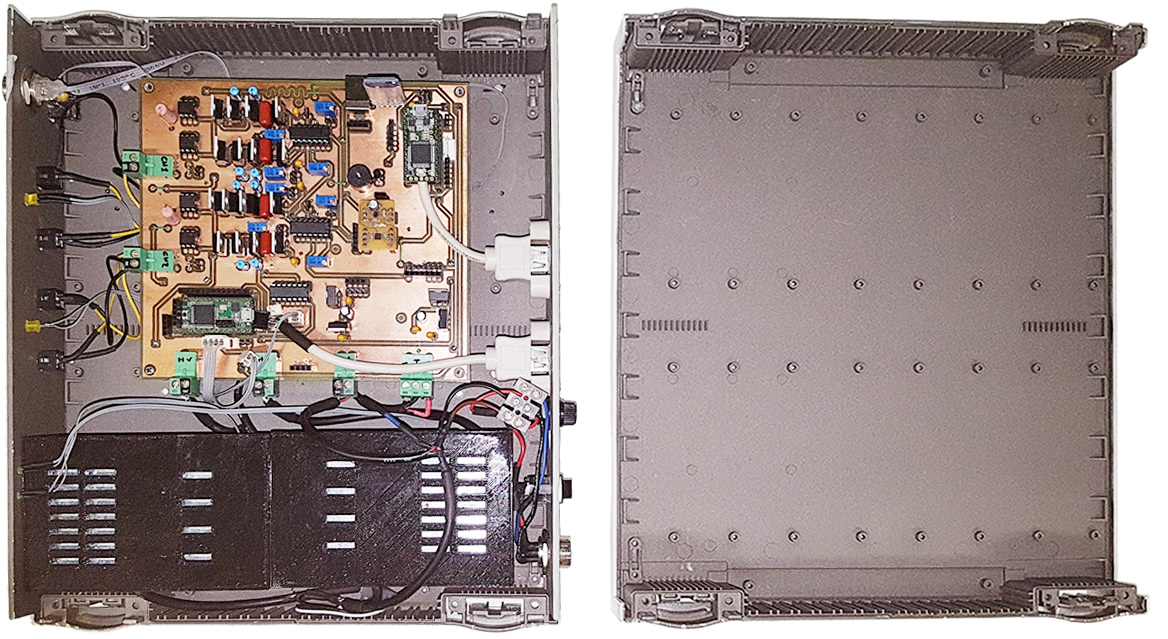
\includegraphics[width=0.9\linewidth]{figs/Fig_c4/c4_f26_dcgp}
    \caption{Disposição dos componentes sistema do eletroestimulador no gabinete.}
    \label{fig:c4_f26_dcgp}
\end{figure*}

%Figura 4.27 – Identificação dos componentes do eletroestimulador.
\begin{figure*}
    \centering %
    \small %
    \def\svgwidth{1\columnwidth}% Código LATEX define o tamanho da figura 
    \import{figs/Fig_c4/}{c4_f27_cie.pdf_tex}
    \caption{Identificação dos componentes do eletroestimulador. a) Vista frontal, b) vista traseira e c) vista isométrica.}
    \label{fig:c4_f27_mpci}
\end{figure*}

Finalmente, na Figura \ref{fig:c4_f28_gfa} é apresentado o gabinete fechado e com seus acessórios. Nesse contexto, o sistema conta com os seguintes acessórios: botão de emergência, cabos dos eletrodos, cabo de extensão do acelerômetro, acelerômetro, fonte medica e tablete (eles são exibidos na Figura 5.1). %%%%%%%%%%%%%%% ojo a la fig

% Figura 4.28 – Gabinete fechado do eletroestimulador à esquerda e eletroestimulador na sua maleta de transporte com todos seus acessórios no lado direito.
\begin{figure*}
    \centering %
    \small %
    \def\svgwidth{1\columnwidth}% Código LATEX define o tamanho da figura 
    \import{figs/Fig_c4/}{c4_f28_gfa.pdf_tex}
    \caption{Gabinete fechado do eletroestimulador à esquerda e eletroestimulador na sua maleta de transporte com todos seus acessórios no lado direito.}
    \label{fig:c4_f28_gfa}
\end{figure*}


\section{SOFTWARE} 
Basicamente, existem dois itens que integram o software do sistema proposto: uma interface gráfica implementada em PC para controlar o eletroestimulador e o firmware da unidade de controle do mesmo.

\subsection{FIRMWARE DO SISTEMA DE ESTIMULAÇÃO} 
Como mencionado nos itens anteriores, a \acrshort{UC} é responsável por gerenciar os recursos e caraterísticas físicas do sistema de eletroestimulação. Desta forma, o fluxograma da Figura \ref{fig:c4_f29_fmw} mostra as caraterísticas principais do firmware da unidade de controle.

% Fluxograma do firmware do estimulador.
\begin{figure*}
    \centering %
    \small %
    \def\svgwidth{1\columnwidth}% Código LATEX define o tamanho da figura 
    \import{figs/Fig_c4/}{c4_f29_fmw.pdf_tex}
    \caption{Fluxograma do firmware do estimulador.}
    \label{fig:c4_f29_fmw}
\end{figure*}

Antes de qualquer procedimento o firmware da \acrshort{UC} ($\mathrm{\mu}$C1\_STIM) realiza algumas fincões iniciais que permitem o correto funcionamento do estimulador. Primeiramente são configurada as portas de comunicação sendo elas Serial (\acrshort{UART}), \acrshort{SPI} e \acrshort{I2C} e inicializa as estruturas de dados que vão guardar las configurações tanto da terapia/treinamento quanto do teste de excitabilidade neuromuscular.  Outra função do $\mathrm{\mu}$C1\_STIM é ativar o módulo seletor de canais para garantir que a saída do \acrshort{EPS} esteja conectada às pré-cargas, ao mesmo tempo em que estabelece um valor de 1mA para cada canal evitando a falta de circulação de corrente no espelho de corrente. Isto é implementado conforme explicado na Seção \ref{sec:cap_sec4.2.6}. Uma função chamada “zeroChannels()” é implementada para o procedimento anterior, a qual é usada em diversas situações. Na sequência de exceção do firmware, é ativada a comunicação Serial com o computador. Assim que uma conexão é estabelecida entre o \acrshort{MC} e \acrshort{PC} é possível o controle do estimulador. Portanto, se não há conexão, nenhum procedimento é realizado, mantendo a saída dos canais ligados na pré-carga.

Em seguida, a lógica do firmware entra em um \textit{loop} baseado em uma máquina de estados. Nela, são esperadas instruções sobre o início de uma sessão. Neste ponto, a \acrshort{UC} recebe informações contendo valores e instruções (tipo se sessão\footnote{Uma sessão pode se caracterizar como um treinamento/terapia ou um teste de excitabilidade neuromuscular} e parâmetros de estimulação) que o usuário estabeleceu na Interface Gráfica de Controle (\acrshort{IGC})de controle do eletroestimulador.

De acordo com o tipo de sessão selecionado é possível iniciar um treinamento/terapia ou um teste de excitabilidade neuromuscular. As sessões de treinamento/terapia são realizadas em malha aberta. Uma sessão de teste é realizada com o apoio do \acrshort{MDM}. Em qualquer caso o firmware executa as instruções requeridas e atualiza os valores dos parâmetros de estimulação ajustados para o canal ou canais que estiverem ativados e retorna informações na \acrshort{IGC} sobre o funcionamento do estimulador e/ou respostas do \acrshort{MDM} na detecção das contrações quando realizado o teste de excitabilidade.

Dentro do firmware existe uma rotina que sempre está em execução. Ela é responsável pela finalização de qualquer tipo de procedimento caso o botão de emergência seja pressionado ou caso a comunicação com a \acrshort{IGC} seja perdida. Isto representa uma medida de segurança implementada no firmware. Finalmente, quando uma sessão termina, ou alguma das condições anteriores acontece, a \acrshort{UC}  envia uma mensagem ao aplicativo informando o resultado da operação (e.g. que a sessão foi finalizada, que o botão de emergência foi apertado, entre outras).

\subsection{INTERFACE GRÁFICA DE CONTROLE DO ESTIMULADOR}
No desenvolvimento das primeiras versões do estimulador, a interface era analógica (Apêndice \ref{ap:ap1}), contando com alguns botões para controlar somente a intensidade e a frequência de um canal. A interface de controle passou de analógica a digital, implementando-a por meio de um aplicativo que é executado em um dispositivo móvel (Apêndice \ref{ap:ap1}). O aplicativo seria usado para maior portabilidade e contava, então, com uma \acrshort{IGC} para o novo sistema de eletroestimulação. Nela, era possível identificar duas operações: terapia (operação em em quatro canais) e diagnóstico (operação em um canal). 

Com a evolução do novo sistema de estimulação foi evidenciado que uma \acrshort{IGC} executada em \acrshort{PC} também atendia as caraterísticas e necessidades do projeto, além de permitir um paralelismos e velocidades maiores na transmissão e recepção de dados entre o estimulador e o \acrshort{PC} conectados via \acrshort{USB}. 

Nesse contexto, a \acrshort{IGC} foi desenvolvida fazendo uso da linguagem Python 3.7 (\textit{Python Software Foundation}, USA) para implementação dos algoritmos e Qt5 (\textit{Qt Company Ltd}, FIN) para implementação da interface gráfica. A Figura \ref{fig:c4_f30_igc} mostra a \acrshort{IGC} do estimulador.

%%%% Figura 4.26 – IGC do estimulador.
\begin{figure*}
    \centering %
    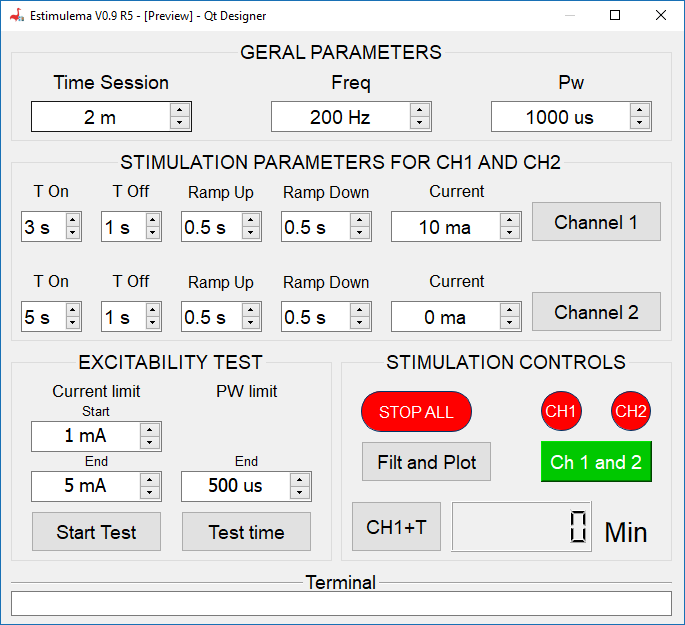
\includegraphics[width=1\linewidth]{figs/Fig_c4/c4_f30_igc}
    \caption{IGC do estimulador.}
    \label{fig:c4_f30_igc}
\end{figure*}

A interface de controle da versão final é multiplataforma podendo se executar em sistemas operacionais (e.g. Windows, Linux ou MAC) que comportem Python 3.7. Além disso, o \acrshort{PC} deve possuir duas portas USB, pois o estimulador usa dois microntroladores ($\mathrm{\mu}$C1\_STIM, $\mathrm{\mu}$C2\_ACEL) para gerencias suas funções. Ademais, para visualizar adequadamente a interface de controle, é necessária uma resolução miníma é 800x600p.

No funcionamento da \acrshort{IGC} estão involucrados tanto os parâmetros de estimulação, como algumas outras caraterísticas adicionais, como: Tempo se sessão, Tempo de estimulação (T-On), Tempo de repouso (T-Off), rampa de subida e rampa de decida.

Desde o ponto de vista do desenvolvimento de software, as soluções escolhidos para \acrshort{IGC} deste trabalho (Python e Qt) são de código aberto e libre utilização.

Finalmente, a interfase de usuário foi desenhada com a finalidade de poder parametrizar cada valor de cada variável e ao mesmo tempo apresentar informações relevantes, como o tempo de estimulação e representação gráfica dos dados adquiridos pelo \acrshort{MDM} imediatamente depois de aplicar o teste de excitabilidade. Um exemplo de representação dos dados adquiridos no \acrshort{MDM}  é apresentado na Figura \ref{fig:c4_f31_xte}.

%%%% Figura 4.26 – IGC do estimulador.
\begin{figure*}
    \centering %
    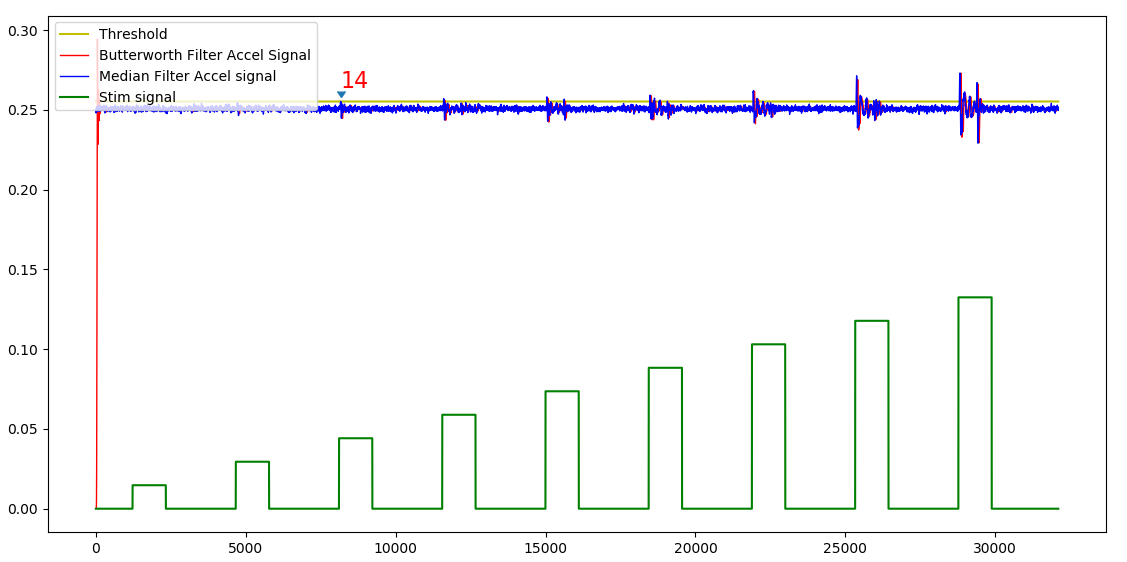
\includegraphics[width=1\linewidth]{figs/Fig_c4/c4_f31_xte}
    \caption{Plot dos dados do teste de excitabilidade.}
    \label{fig:c4_f31_xte}
\end{figure*}
